\clearpage

\section{X. Программа экзамена в 2024/2025}


\begin{enumerate}
    \item Выборочная функция распределения. Теоремы Гливенко-Кантелли и Колмогорова.

    \Def \hyperlink{selective_distribution_function}{Выборочной функцией распределения} $F^*(x)$ называется функция 
    
    $F^*(x) = \frac{\text{число данных } x_i < x}{n}$

    \begin{MyTheorem}
        \Ths Выборочная функция распределения поточечно сходится к теоретической функции распределения:

        \[\forall y \in \Real F^*(y) \overset{p}{\longrightarrow} F(y)\]
    \end{MyTheorem}

    \begin{MyTheorem}
        \ThNs{Гливенко-Кантелли} $\sup_{x \in \Real} |F^*(x) - F(x)| \overset{p}{\longrightarrow} 0$
    \end{MyTheorem}

    \begin{MyTheorem}
        \ThNs{Колмогорова} $\sqrt{n} \sup_{x \in \Real} |F^*(x) - F(x)| \rightrightarrows K$ - распределение Колмогорова с 
        функцией распределения $F_K(x) = \sum_{j = -\infty}^{\infty} (-1)^j e^{-2 j^2 x^2}, \ x \in [0;\infty)$
    \end{MyTheorem}

    \item Вариационный и интервальный вариационный ряды. Полигон и гистограмма, ее свойства.

        
    \hyperlink{initial_data_processing}{Начальная обработка статданных}

    \begin{enumerate}
        \item Ранжирование данных - упорядочиваем выборки по возрастанию. В результате получаем вариационный ряд $\vec{X} = (X_{(1)}, X_{(2)}, \dots, X_{(n)})$

        $X_{(1)} = \min X_i; \quad X_{(n)} = \max X_i$

        $X_{(i)} = i$-ая порядковая статистика

        \item Объединим повторяющиеся данные - получаем т.н. частотный вариационный ряд

        \begin{tabular}{c|c|c|c|c}
            $X_i$ & $X_{(1)}$ & \dots & $X_{(r)}$ & $\sum$ \\ 
            \hline
            $n_i$ & $n_1$ & \dots & $n_r$ & $n$ \\ 
        \end{tabular}

        Иногда часть данных отбрасывается сверху и снизу (по 5, по 10, по 5\% и так далее), чтобы сделать выборку репрезентативной

        Тогда $\overline{x} = \frac{1}{n} \sum X_i n_i$, $D^* = \frac{1}{n} \sum (X_i - \overline{x})^2 n_i$
        
        \item Чтобы уменьшить количество вычислений или сделать гистограмму, делают интервальный вариационный ряд: 
        разбиваем данные на интервалы и считаем, сколько данных $n_i$ попало в интервал. 

        Тогда $n_i$ - частота интервала $A_i$

        Есть два основные способа разбиения на интервалы: 

        \begin{enumerate}
            \item Интервалы одинаковой длины
            \item Равнонаполненные интервалы (в каждом интервале примерно одинаковое количество данных)
        \end{enumerate}

        Число интервалов $K$ такое, что $\frac{K(n)}{n} \longrightarrow 0$ и $K(n) \underset{n \to \infty}{\longrightarrow} \infty$

        Обычно применяют формулу Стерджесса $K \approx 1 + \log_2 n$ или $K \approx \sqrt[3]{n}$

        Пусть получили интервальный вариационный ряд

        \begin{tabular}{c|c|c|c|c|c}
            интервалы & $[a_0; a_1)$ & $[a_1; a_2)$ & \dots & $[a_{K - 1}; a_K]$ & $\sum$ \\ 
            \hline
            частоты & $n_1$ & $n_2$ & \dots & $n_K$ & $n$ \\ 
        \end{tabular}
    \end{enumerate}

    \smallvspace
        
    \begin{multicols}{2}
        \begin{itemize}
            \item Гистограмма

            Строится ступенчатая фигура из прямоугольников, основание $i$-ого прямоугольника - интервал, 
            высота прямоугольника - $\frac{n_i}{n l_i}$, где $l_i$ - длина интервала. 
            Визуально можно сделать гипотезу, как ведет себя распределение. 

            \begin{center}
                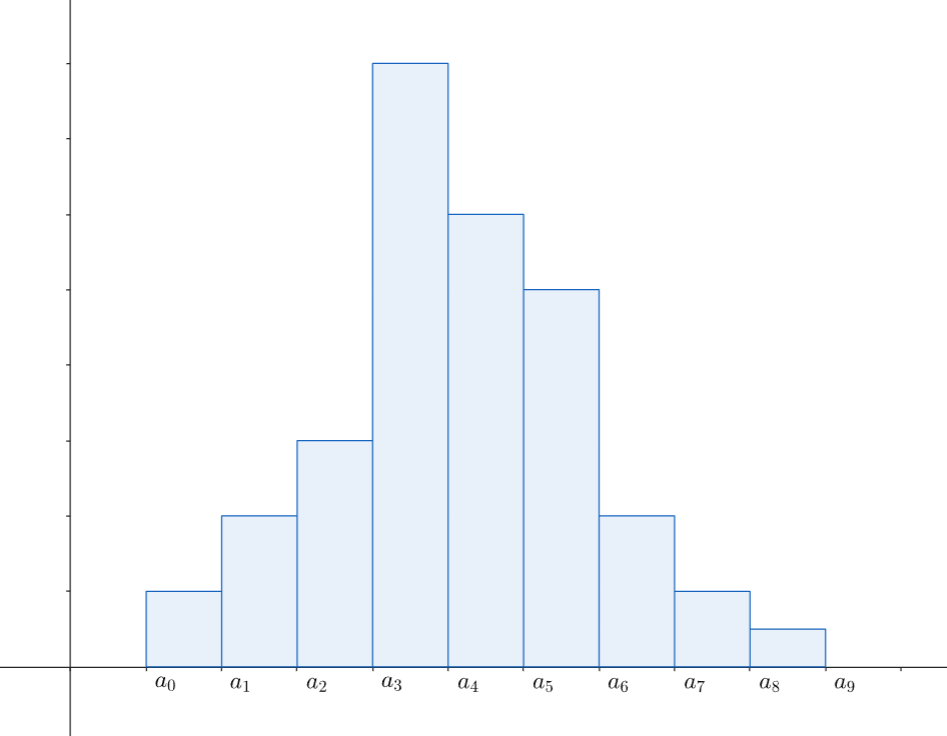
\includegraphics[width=0.4\textwidth]{mathstat/images/mathstat_2025_02_11_1}
            \end{center}

            \item Полигон

            На оси абсцисс отмечаем значения частотного вариационного ряда, по оси ординат - их частоты. 
            Получившиеся точки соединяем отрезками

            \begin{center}
                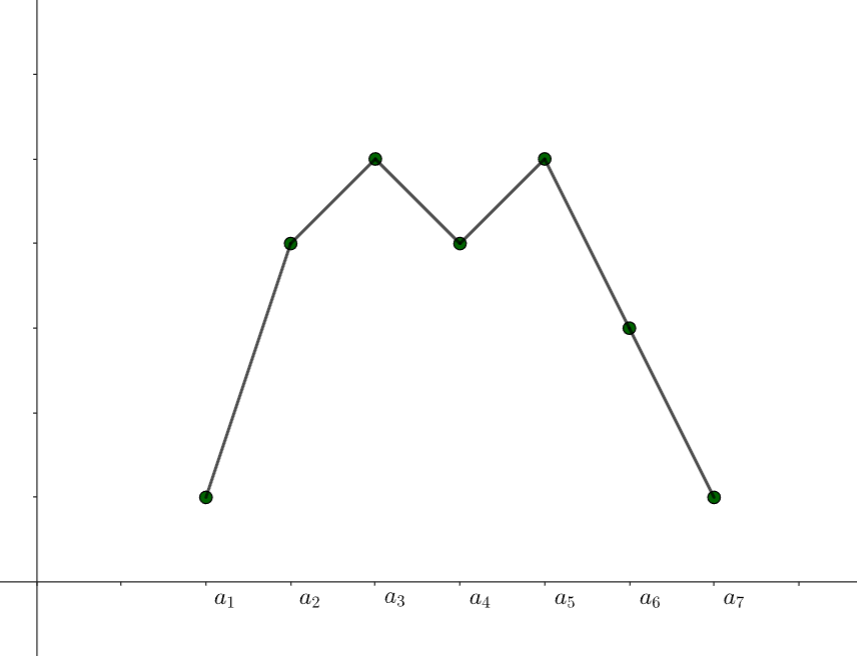
\includegraphics[width=0.4\textwidth]{mathstat/images/mathstat_2025_02_11_2}
            \end{center}
        \end{itemize}
    \end{multicols}

    \item Точечные оценки. Их свойства: состоятельность, несмещенность, эффективность.

    Пусть имеется выборка $\vec{X} = (X_1, X_2, \dots, X_n)$ объемом $n$. Пусть требуется найти приближенную оценку $\theta^*$ неизвестного параметра $\theta$. Находим ее при помощи некоторой функции обработки данных $\theta^* = \theta^*(X_1, \dots, X_n)$
    
    \Defs Такая функция называется статистикой
    
    \Defs А оценка $\theta^*$ называется \hyperlink{point_estimation}{точечной оценкой}

    \Defs Статистика $\theta^* = \theta^*(X_1, \dots, X_n)$ неизвестного параметра называется
    \textbf{состоятельной}, если $\theta^* \overset{p}{\longrightarrow} \theta$ при $n \to \infty$

    \Defs Оценка $\theta^*$ параметра $\theta$ называется \textbf{несмещенной}, если 
    математическое ожидание $E \theta^* = \theta$
        
    \Notas Оценка $\theta^*$ называется асимптотически несмещенной, если 
    $E \theta^* \overset{p}{\longrightarrow} \theta$ при $n \to \infty$

    \Defs Оценка $\theta^*_1$ не хуже $\theta^*_2$, если $E (\theta^*_1 - \theta)^2 \leq E (\theta^*_2 - \theta)^2$.
    Или, если $\theta^*_1$ и $\theta^*_2$ несмещенные, то $D \theta^*_1 \leq D \theta^*_2$

    \Defs Оценка $\theta^*$ называется \textbf{эффективной}, если она не хуже всех остальных оценок

    \Notas Не существует эффективной оценки в классе всех возможных оценок

    \begin{MyTheorem}
        \Ths В классе несмещенных оценок существует эффективная оценка
    \end{MyTheorem}

    \Defs Оценка $\theta^*$ параметра $\theta$ называется асимптотически нормальной, если 
    $\sqrt{n} (\theta^* - \theta) \rightrightarrows N(0, \sigma^2 (\theta))$ при $n \to \infty$

    \item Точечные оценки моментов. Свойства оценок математического ожидания и дисперсии.

    \hyperlink{moments_point_estimation}{Точечные оценки моментов}:

    \Defs Выборочным средним $\overline{x}$ называется величина $\overline{x} = \frac{1}{n} \sum_{i = 1}^n X_i$

    \Defs Выборочной дисперсией $D^*$ называется величина $D^* = \frac{1}{n} \sum_{i = 1}^n (X_i - \overline{x})^2$

    \Defs Исправленной дисперсией $S^2$ называется величина $S^2 = \frac{n}{n - 1} D^* = \frac{1}{n - 1} \sum_{i = 1}^n (X_i - \overline{x})^2$

    \Defs Выборочным средним квадратическим отклонением называется величина $\sigma^* = \sqrt{D^*}$

    \Defs Исправленным средним квадратическим отклонением называется величина $S = \sqrt{S^2}$

    \Defs Выборочным $k$-ым моментом называется величина $\overline{x^k} = \frac{1}{n} \sum_{i = 1}^n X_i^k$

    \Defs Модой $\mathrm{Mo}^*$ называется варианта $x_k$ с наибольшей частотой $n_k = \max_i (n_1, n_2, \dots, n_m)$

    \Defs Выборочной медианой $\mathrm{Me}^*$ называется варианта $x_i$ в середине вариационного ряда $\begin{cases}\mathrm{Me}^* = 
    X_{(k)}, & \text{если } n = 2k - 1 \\ \frac{X_{(k)} + X_{(k + 1)}}{2}, & \text{если } n = 2k\end{cases}$
    
    \begin{MyTheorem}
        \Ths $\overline{x}$ - состоятельная несмещенная оценка теоретического матожидания $EX = a$
    
        1) $E \overline{x} = a$
    
        2) $\overline{x} \overset{p}{\longrightarrow} a$ при $n \to \infty$
    \end{MyTheorem}
    
    \begin{MyTheorem}
        \Ths Выборочный $k$-ый момент является состоятельной несмещенной оценкой теоретического $k$-ого момента
    
        1) $\overline{E X^k} = E X^k$
    
        2) $\overline{X^k} \overset{p}{\longrightarrow} X^k$
    \end{MyTheorem}
    
    \begin{MyTheorem}
        \Ths Выборочной дисперсией $D^*$ и $S^2$ являются состоятельными оценками теоретической дисперсией, при этом $D^*$ - смещенная оценка, а $S^2$ - несмещенная оценка
    \end{MyTheorem}

    \item Метод моментов. Пример.

    \hyperlink{method_of_moments}{Метод моментов}: пусть имеется выборка объема $n$ неизвестного распределения, но известного типа,
    которое задается $k$ параметрами: $\theta = (\theta_1, \theta_2, \dots, \theta_k)$. Требуется дать оценки данным
    неизвестным параметрам

    Идея метода состоит в том, что сначала находим оценки $k$ моментов, а затем с помощью теоретических формул
    из теории вероятности даем оценки этих параметров

    Пусть $\vec{X}$ - выборка из абсолютно непрерывного распределения $F_\theta$ с плотностью известного типа, 
    которая задается $k$ параметрами $f_\theta (x, \theta_1, \dots, \theta_k)$

    Тогда теоретические моменты находим по формуле $m_i = \int_{-\infty}^{\infty} x^i f_\theta (x, \theta_1, \dots, \theta_k) dx = h_i(\theta_1, \dots, \theta_n)$

    Получаем систему из $k$ уравнений с $k$ неизвестными. В эти уравнения подставляем найденные оценки
    моментов и, решая получившуюся систему уравнений, находим нужные оценки параметров

    $\begin{cases}
    \overline{x} = h_1(\theta_1^*, \dots, \theta_n^*) \\ 
    \overline{x^2} = h_2(\theta_1^*, \dots, \theta_n^*) \\ 
    \dots \\
    \overline{x^k} = h_k(\theta_1^*, \dots, \theta_n^*) \\ 
    \end{cases}$

    \Ex Пусть $X \in U(a, b)$. Обработав статданные, нашли оценки первого и второго моментов: $\overline{x} = 2.25; \overline{x^2} = 6.75$

    Нужно найти оценки параметров $a^*, b^*$

    $EX = \int_a^b x \frac{1}{b - a} dx = \frac{a + b}{2}$

    $EX = \int_a^b x^2 \frac{1}{b - a} dx = \frac{a^2 + ab + b^2}{3}$

    Получаем:

    $\begin{cases}
        \overline{x} = \frac{a^* + b^*}{2} \\ 
        \overline{x^2} = \frac{a^*^2 + a^* b^* + b^*^2}{3} \\ 
    \end{cases} \Longleftrightarrow \begin{cases}
        a^* + b^* = 4.5 \\ 
        a^*^2 + a^* b^* + b^*^2 = 20.25 \\ 
    \end{cases} \Longleftrightarrow \begin{cases}
        a^* + b^* = 4.5 \\ 
        a^* b^* = 0 \\ 
    \end{cases} \Longleftrightarrow \begin{cases}
        a^* = 0 \\ 
        b^* = 4.5 \\ 
    \end{cases}$

    \item Метод максимального правдоподобия. Пример.

    \hyperlink{maximum_likelihood_estimation}{Метод максимального правдоподобия}: пусть имеется выборка $\vec{X} = (X_1, \dots, X_n)$ из распределения известного типа, определяемого неизвестными параметрами 
    $\theta = (\theta_1, \dots, \theta_n)$

    Идея метода состоит в следующем: подбираем параметры таким образом, чтобы вероятность получения
    данной выборки при случайном эксперименте была наибольшей.

    Если распределение дискретное, то $P_{\theta} (X_1 = x_1, X_2 = x_2, \dots, X_n = x_n) = P(X_1 = x_1) \dots P(X_n = x_n)$

    \Defs Функцией правдоподобия $L(\vec{X}, \theta)$ называется функция $L(\vec{X}, \theta) = P(X_1 = x_1) \dots P(X_n = x_n) = \prod_{i = 1}^n P(X_i = x_i)$ при дискретном распределении

    и $L(\vec{X}, \theta) = f_\theta(x_1) \dots f_\theta(x_n) = \prod_{i = 1}^n f_\theta(x_i)$ в абсолютно непрерывном распределении

    \Defs Логарифмической функцией правдоподобия называется функция $\ln L(\vec{X}, \theta)$

    \Notas Так как $y = \ln x$ возврастающая функция, точки максимума совпадают, а такую функцию правдоподобия становится легче дифференцировать

    \Defs Оценкой максимального правдоподобия $\hat{\theta}$ называется значение $\theta$, при котором функция правдоподобия 
    $L(\vec{X}, \theta)$ достигает наибольшего значения (при фиксированных значениях выборки)

    \Ex Пусть $\vec{X} = (X_1, \dots, X_n)$ - выборка из распределения Пуассона $\Pi_\lambda$ с неизвестным $\lambda > 0$

    \Mems Для распределения Пуассона $P(X = x_i) = \frac{\lambda^{x_i}}{x_i!} e^{-\lambda}$
    
    Получаем функцию максимального правдоподобия $L(\vec{X}, \lambda) = \prod_{i = 1}^n \frac{\lambda^{x_i}}{x_i!} e^{-\lambda} = 
    \frac{\lambda^{\sum_{i = 1}^n x_i}}{\prod_{i = 1}^n x_i!} e^{-n\lambda} = \frac{\lambda^{n \overline{x}}}{\prod_{i = 1}^n x_i!} e^{-n\lambda}$
    
    $\ln L(\vec{X}, \lambda) = n \overline{x} \ln \lambda - \ln \prod_{i = 1}^n x_i! - n\lambda$
    
    $\frac{\partial \ln L}{\partial \lambda} = \frac{n \overline{x}}{\lambda} - n = 0 \Longrightarrow \hat{\lambda} = \overline{x}$ - оценка максимального правдоподобия
    
    Убедимся, что этот экстремум - максимум: $\frac{\partial^2 \ln L}{\partial \lambda^2} = -\frac{n \overline{x}}{\lambda} < 0 \Longrightarrow \hat{\lambda} = \overline{x}$ - точка максимума
    
    \item Информация Фишера. Неравенство Рао-Крамера (без док-ва).

    Пусть $X \in F_\theta$ - семейство распределений с параметром $\theta \in \Real$

    \Def Носителем семейства распределений $F_\theta$ называется множество $C \subset \Real$
    такое, что $P(X \in C) = 1 \ \forall X \in F_\theta$

    $f_\theta(x) = \begin{cases}
        \text{плотность } f_\theta(x) \text{ при непрерывном распределении} \\
        P_\theta(X = x) \text{ при дискретном распределении}
    \end{cases}$

    \Def \hyperlink{fishers_information}{Информацией Фишера} $I(\theta)$ семейства распределений $F_\theta$ называется величина 
    $I(\theta) = E\left(\frac{\partial}{\partial \theta} \ln f_\theta(X)\right)^2$ при условии, что
    она существует

    \Def Семейство распределений $F_\theta$ называется регулярным, если:

    \begin{itemize}
        \item существует носитель $C$ семейства $F_\theta$ такой, что $\forall x \in C \ $ функция $\ln f_\theta(x)$ непрерывно дифференцируема по $\theta$
        \item информация Фишера $I(\theta)$ существует и непрерывна по $\theta$
    \end{itemize}

    \begin{MyTheorem}
        \ThNs{\hyperlink{rao_kramer_inequality}{Неравенство Рао-Крамера}} Пусть $(X_1, \dots, X_n)$ - выборка объема $n$ из регулярного семейства $F_\theta$,

        $\theta^* = \theta^*(X_1, \dots, X_n)$ - несмещенная оценка параметра $\theta$, дисперсия которой
        $D\theta^*$ ограничена в любой замкнутой ограниченной области параметра $\theta$

        Тогда \fbox{$D\theta^* \geq \frac{1}{n I(\theta)}$}
    \end{MyTheorem}

    \underline{Следствие}: если при данных услових получили $D\theta^* = \frac{1}{n I(\theta)}$, то оценка $\theta^*$ является эффективной 
    (то есть дальше улучшать уже некуда)

    \item Основные распределения математической статистики: хи-квадрат, Стьюдента, Фишера-Снедекора. Их свойства.

    \Def Распределение \enquote{хи-квадрат} $H_n$ со степенями свободы $n$ называется распределение
    суммы квадратов независимых стандартных нормальных величин: $\chi^2_n = X_1^2 + X_2^2 + \dots + X_n^2$, 
    где $X \in N(0, 1)$ и независимы

    \underline{Свойства}

    \begin{enumerate}
        \item $E\chi^2_n = n$

        \begin{MyProof}
            Так как $\forall i \ X_i \in N(0, 1)$, то $E X_i^2 = D X_i^2 + (EX_i)^2 = 1 \Longrightarrow E(X_i^2 + \dots X_n^2) = \sum_{i = 1}^n E X_i^2 = n$
        \end{MyProof}

        \item Устойчивость относительно суммирования: если $X \in H_n$, $Y \in H_m$, независимы, то $X + Y \in H_{n + m}$ (по определению) 


        \item $\frac{\chi_k^2}{k} \overset{p}{\underset{k \to \infty}{\longrightarrow}} 1$ (по Закону Больших Чисел)
    \end{enumerate}

    \Def Пусть $X_0, X_1, \dots, X_k$ - независимые стандартные нормальные величины. 
    Распределением Стьюдента $T_k$ с $k$ степенями свободы называется распределение случайной величины 
    $t_k = \frac{X_0}{\sqrt{\frac{1}{k} (X_1^2 + \dots + X_k^2)}} = \frac{X_0}{\sqrt{\frac{\chi_k^2}{k}}}$

    \underline{Свойства}

    \begin{enumerate}
        \item $Et_k = 0$ - в силу симметрии

        \item $t_k \rightrightarrows N(0, 1)$ (на практике при $k \geq 100$ распределение Стьюдента можно считать стандартным нормальным)
    \end{enumerate}

    \Def Распределением Фишера-Снедекера $F_{n,m}$ (другое название - F-распределение) со степенями свободы $n$ и $m$ называется распределение случайной величины 
    $f_{n,m} = \frac{\frac{\chi^2_n}{n}}{\frac{\chi^2_m}{m}}$, где $\chi_n^2$ и $\chi_m^2$ - независимые случайные величины с распределением \enquote{хи-квадрат}

    \underline{Свойства}

    \begin{enumerate}
        \item $E f_{n,m} = \frac{n}{n - 2}$

        \item $f_{n,m} \overset{p}{\underset{n, m \to \infty}{\longrightarrow}} 1$
    \end{enumerate}

    \item Линейные преобразования нормальных выборок. Теорема об ортогональном преобразовании.

    \Def Пусть случайный вектор $\vec \xi = \begin{pmatrix}\xi_1 \\ \vdots \\ \xi_n\end{pmatrix}$ имеет вектор средних 
    $\vec a = E \vec \xi$, $K$ - симметричная положительно определенная матрица. Вектор $\vec \xi$ 
    имеет нормальное распределение в $\Real^n$ с параметрами $\vec a$ и $K$, если его плотность 
    $f_{\vec \xi} (\vec X) = \frac{1}{\left(\sqrt{2\pi}\right)^n \sqrt{\det K}} e^{-\frac{1}{2} (\vec X - \vec a)^T K^{-1} (\vec X - \vec a)}$


    \underline{Свойства}

    \begin{enumerate}
        \item Матрица $K = D \vec \xi = \left(\mathrm{cov} (\xi_i, \xi_j)\right)$ - матрица ковариаций

        \item При $\vec a = \vec 0$ и $K = E$ имеем вектор из независимых стандартных нормальных величин

        \begin{MyProof}
            При $\vec a = \vec 0$ и $K = E$: $f_{\vec \xi} (X_1, \dots, X_n) = \frac{1}{\left(\sqrt{2\pi}\right)^n} 
            e^{-\frac{1}{2} \begin{pmatrix}X_1 & \dots & X_n\end{pmatrix} E \begin{pmatrix}X_1 & \dots & X_n\end{pmatrix}^T} = 
            \frac{1}{\left(\sqrt{2\pi}\right)^n} e^{-\frac{1}{2} (X_1^2 + \dots + X_n^2)} = 
            \frac{1}{\sqrt{2\pi}} e^{-\frac{1}{2} X_1^2} + \dots + \frac{1}{\sqrt{2\pi}} e^{-\frac{1}{2} X_n^2}$

            Так как плотность распалась на произведение плотностей стандартного нормального распределение, то все компоненты имеют стандартное нормальное распределение
        \end{MyProof}

        \item $\letsymbol \vec X$ - стандартный нормальный вектор, $B$ - невырожденная матрица, 
        тогда вектор $\vec Y = B \vec X + \vec a$ имеет многомерное нормальное распределение с параметрами $\vec a$ и $K = B B^T$

        \item $\letsymbol \vec Y \in N(\vec a, K)$. Тогда вектор $\vec X = B^{-1} (\vec Y - \vec a)$ - стандартный нормальный вектор, где $B = \sqrt{K}$

        \underline{Следствие}. Эквивалентное определение: Многомерное нормальное распределение - это то, которое получается из
        стандартного нормального вектора при помощи невырожденного преобразования и сдвига

        \item $\letsymbol \vec X$ - стандартный нормальный вектор, $C$ - ортогональная матрица. Тогда $\vec Y = C \vec X$ - стандартный нормальный вектор

        \begin{MyProof}
            Так как $C$ - ортогональная, то $C^T = C^{-1}$. Тогда по третьему свойству $K = C C^T = E$, а по второму свойству $\vec Y$ - стандартный нормальный вектор
        \end{MyProof}

        \item $\letsymbol$ случайный вектор $\xi \in N(\vec a, K)$.
        Тогда его координаты независимы тогда и только тогда, когда они не коррелированы (то есть матрица ковариаций $K$ диагональная)

        % какого распределения величины
        \underline{Следствие}. Если плотность совместного распределения случайных величин $\xi$ и $\eta$ ненулевая, то они независимы тогда и только тогда, 
        когда их коэффициент корреляции равен нулю
    \end{enumerate}

    \item Лемма Фишера.

    \begin{MyTheorem}
        \Ths{\hyperlink{fishers_lemma}{Лемма Фишера}} Пусть вектор $\vec X$ - стандартный нормальный вектор, $C$ - ортогональная матрица, $\vec Y = C \vec X$.
        Тогда $\forall 1 \leq k \leq n - 1 \ $ случайная величина $T(\vec X) = \sum_{i = 1}^n X_i^2 - Y_1^2 - Y_2^2 - \dots Y_k^2$ 
        не зависит от $Y_1, Y_2, \dots, Y_k$ и имеет распределение \enquote{хи-квадрат} со степенями свободы $n - k$
    \end{MyTheorem}

    \begin{MyProof}
        Так как $C$ - ортогональное преобразование, то $\|\vec X\| = \|\vec Y\|$, то есть $\sum_{i = 1}^n X^2_i = \sum_{i = 1}^n Y^2_i \Longrightarrow
        T(\vec X) = \sum_{i = 1}^n X_i^2 - Y_1^2 - Y_2^2 - \dots Y_k^2 = Y^2_{k + 1} + \dots + Y^2_{n}$

        Согласно свойству 5 $Y_i \in N(0, 1)$ и независимы, то по определению \enquote{хи-квадрат} $T(\vec X) \in H_{n - k}$ и не зависит от $Y_1, \dots, Y_k$
    \end{MyProof}

    \item Основная теорема о связи точечных оценок нормального распределения и основных распределений статистики.

    \begin{MyTheorem}
        \Ths Пусть $(X_1, \dots, X_n)$ - выборка из нормального распределения $N(a, \sigma^2)$, $\overline{x}$ - выборочное среднее, $S^2$ - исправленная дисперсия.

        Тогда справедливы следующие высказывания:

        \begin{enumerate}
            \item $\sqrt{n} \frac{\overline{x} - a}{\sigma} \in N(0, 1)$
            
            \item $\sum_{i = 1}^n \frac{(X_i - a)^2}{\sigma^2} \in H_n$
            
            \item $\sum_{i = 1}^n \frac{(X_i - \overline{x})^2}{\sigma^2} = \frac{n D^*}{\sigma^2} = \frac{(n - 1) S^2}{\sigma^2} \in H_{n - 1}$

            \item $\sqrt{n} \frac{\overline{x} - a}{S} \in T_{n - 1}$
            
            \item $\overline{x}$ и $S^2$ независимы
        \end{enumerate}
    \end{MyTheorem}

    \item Квантили распределений (оба определения). Функции для их вычисления в EXEL.

    Пусть нам дано распределение абсолютно непрерывное, и $F(x)$ - функция распределения

    \DefN{1} Число $t_\gamma$ называется \hyperlink{quantile_distribution}{квантилем распределения} уровня $\gamma$, если значения
    функции распределения $F(t_\gamma) = \gamma$ или $P(X < t_\gamma) = \gamma$ ($t_\gamma = F^{-1}(\gamma)$)

    % https://www.geogebra.org/calculator/ezemup66

    \begin{center}
        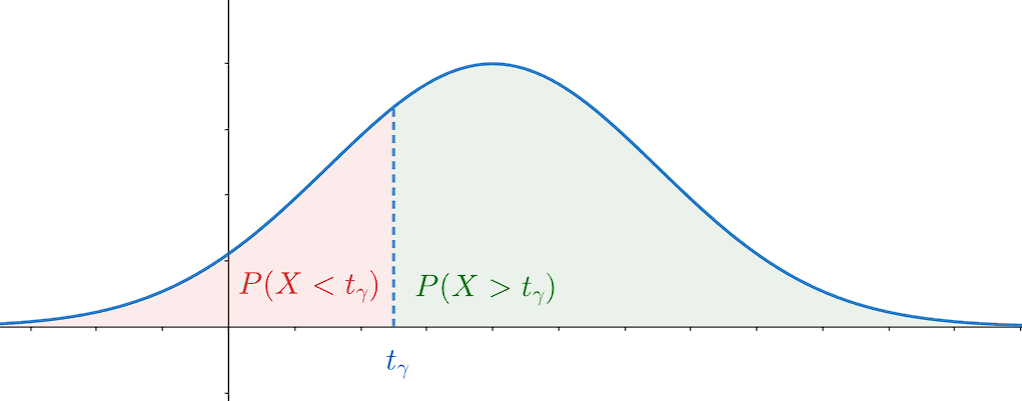
\includegraphics[width=7cm]{mathstat/images/mathstat_2025_03_11_1}
    \end{center}

    \Ex Медиана - квантиль уровня $\frac{1}{2}$

    \DefN{2} Число $t_\alpha$ называется квантилем уровня значимости $\alpha$, если
    $P(X > t_\alpha) = \alpha$ или $F(t_\alpha) = 1 - \alpha$

    Ясно, что $\gamma = 1 - \alpha$

    В Excel для вычисления квантилей распределения используются обратные функции распределения: \verb|НОРМ.СТ.ОБР()|, \verb|F.ОБР()|, \verb|ХИ2.ОБР()|, \verb|СТЬЮДЕНТ.ОБР()|

    \item Интервальные оценки. Определения, смысл, терминология.

    Недостатки точечных оценок - неизвестно насколько они далеки от реального значения параметра и 
    насколько им можно доверять. Особенно это заметно при малых выборках. Поэтому мы указываем интервал, в котором 
    лежит этот параметр с заданной вероятностью (надежностью) $\gamma$. Такие оценки называются интервальными 
    (доверительными)

    \Def \hyperlink{interval_estimation}{Интервал} $(\theta^-_\gamma; \theta^+_\gamma)$ называется доверительным интервалом параметра $\theta$
    надежности $\gamma$, если вероятность $P(\theta^-_\gamma < \theta < \theta^+_\gamma) = \gamma$
    
    \Nota Если имеем дискретную случайную величину, то $P(\theta^-_\gamma < \theta < \theta^+_\gamma) \geq \gamma$
    
    \Notas Так как параметр $\theta$ - константа, то бессмысленно говорить о его попадании в интервал. Правильно: 
    доверительный интервал накрывает параметр $\theta$ с вероятностью $\gamma$
    
    \NotaN{1} $\alpha = 1 - \gamma$ называется уровнем значимости доверительного интервала
    
    \NotaN{2} Обычно пытаются строить симметричный доверительный интервал относительно несмещенной оценки $\theta^*$
    
    \NotaN{3} Возникает вопрос, какой уровень $\gamma$ выбрать для исследования.
    Стандартные уровени надежности $\gamma$: $0.9, \ 0.95, \ 0.99, \ 0.999$. Самый мейнстримный - $0.95$. 
    В малых выборках используют $0.9$

    \item Доверительный интервал для математического ожидания нормального распределения при известном $\sigma$.

    \hyperlink{confidence_interval_for_a_known_sigma}{Доверительный интервал для параметра $a$ при известном значении $\sigma^2$}

    По пункту 1 из теоремы $\sqrt{n} \frac{\overline{x} - a}{\sigma} \in N(0, 1)$ 

    $P\left(-t_\gamma < \sqrt{n} \frac{\overline{x} - a}{\sigma} < t_\gamma\right) = 
    P\left(\left|\sqrt{n} \frac{\overline{x} - a}{\sigma}\right| < t_\gamma\right) = 2F_0 (t_\gamma) - 1 = \gamma$

    $F_0(t_\gamma) = \frac{1 + \gamma}{2} \Longrightarrow t_\gamma$ - квантиль уровня 
    $\frac{1 + \gamma}{2}$ для $N(0, 1)$, где
    $F_0(x) = \frac{1}{\sqrt{2\pi}} \int_{-\infty}^{\infty} e^{-\frac{z^2}{2}} dz$

    Решая неравенство, получаем $-t_\gamma < \sqrt{n} \frac{\overline{x} - a}{\sigma} < t_\gamma$

    $-t_\gamma \frac{\sigma}{\sqrt{n}} < \overline{x} - a < t_\gamma \frac{\sigma}{\sqrt{n}}$

    $\overline{x} - t_\gamma \frac{\sigma}{\sqrt{n}} < a < \overline{x} + t_\gamma \frac{\sigma}{\sqrt{n}}$ - 
    симметричный интервал относительно $\overline{x}$

    Доверительный интервал надежности $\gamma$: $\left(\overline{x} - t_\gamma \frac{\sigma}{\sqrt{n}}, 
    \overline{x} + t_\gamma \frac{\sigma}{\sqrt{n}}\right)$, 
    где $t_\gamma$ - квантиль $N(0, 1)$ уровня $\frac{1 + \gamma}{2}$

    \item Доверительный интервал для математического ожидания нормального распределения при неизвестном $\sigma$.

    \hyperlink{confidence_interval_for_a_unknown_sigma}{Доверительный интервал для параметра $a$ при неизвестном $\sigma^2$}

    Из пункта 4 из теоремы $\sqrt{n} \frac{\overline{x} - a}{S} \in T_{n - 1}$

    $P\left(-t_\gamma < \sqrt{n} \frac{\overline{x} - a}{S} < t_\gamma\right) = P\left(\left|\sqrt{n} \frac{\overline{x} - a}{S}\right| < t_\gamma\right) = 2F_{T_{n - 1}}(t_\gamma) = \gamma$

    $F_{T_{n - 1}}(t_\gamma) = \frac{1 + \gamma}{2} \Longrightarrow t_\gamma$ - квантиль $T_{n - 1}$ уровня 
    $\frac{1 + \gamma}{2}$

    Аналогично с примером выше получаем интервал $\left(\overline{x} - t_\gamma \frac{S}{\sqrt{n}}, 
    \overline{x} + t_\gamma \frac{S}{\sqrt{n}}\right)$, 
    где $t_\gamma$ - квантиль $T_{n - 1}$ уровня $\frac{1 + \gamma}{2}$

    \item Доверительный интервал для дисперсии нормального распределения при неизвестном $a$.

    \hyperlink{confidence_interval_for_sigma_unknown_a}{Доверительный интервал для параметра $\sigma^2$ при неизвестном $a$}

    По пункту 3 из теоремы $\sum_{i = 1}^n \left(\frac{X_i - \overline{x}}{\sigma}\right)^2 = \frac{(n - 1)S^2}{\sigma^2} = 
    \frac{nD^*}{\sigma^2} \in H_{n - 1}$

    Пусть $\chi_1^2$ и $\chi_2^2$ - квантили $H_{n - 1}$ уровней $\frac{1 - \gamma}{2}$ и $\frac{1 + \gamma}{2}$

    Тогда $P\left(\chi_1^2 < \frac{(n - 1)S^2}{\sigma^2} < \chi_2^2\right) = F_{H_{n - 1}}(\chi_1^2) - F_{H_{n - 1}}(\chi_2^2) = \frac{1 - \gamma}{2} - \frac{1 + \gamma}{2} = \gamma$

    $\chi_1^2 < \frac{(n - 1)S^2}{\sigma^2} < \chi_2^2$

    $\frac{1}{\chi_2^2} < \frac{\sigma^2}{(n - 1)S^2} < \frac{1}{\chi_1^2}$

    $\frac{(n - 1)S^2}{\chi_2^2} < \sigma^2 < \frac{(n - 1)S^2}{\chi_1^2}$ или 
    $\frac{nD^*}{\chi_2^2} < \sigma^2 < \frac{nD^*}{\chi_1^2}$

    Получаем интервал $\left(\frac{(n - 1)S^2}{\chi_2^2}, \frac{(n - 1)S^2}{\chi_1^2}\right)$, где $\chi_1^2$ и $\chi_2^2$ - квантили $H_{n - 1}$ уровней $\frac{1 - \gamma}{2}$ и $\frac{1 + \gamma}{2}$

    \Nota Данный интервал не симметричен относительно неизвестного параметра $\sigma^2$

    \item Доверительный интервал для дисперсии нормального распределения при известном $a$.

    \hyperlink{confidence_interval_for_sigma_known_a}{Доверительный интервал для параметра $\sigma^2$ при известном $a$}

    По пункту 2 из теоремы $\sum_{i = 1}^n \left(\frac{X_i - a}{\sigma}\right)^2 = \frac{n \tilde{\sigma^2}}{\sigma^2} \in H_{n - 1}$
    
    Пусть $\chi_1^2$ и $\chi_2^2$ - квантили $H_{n}$ уровней $\frac{1 - \gamma}{2}$ и $\frac{1 + \gamma}{2}$

    Тогда $P\left(\chi_1^2 < \frac{n \tilde{\sigma^2}}{\sigma^2} < \chi_2^2\right) = F_{H_{n}}(\chi_1^2) - F_{H_{n}}(\chi_2^2) = \frac{1 - \gamma}{2} - \frac{1 + \gamma}{2} = \gamma$

    Аналогично получаем интервал $\left(\frac{n \tilde{\sigma^2}}{\chi_2^2}, \frac{n \tilde{\sigma^2}}{\chi_1^2}\right)$, 
    где $\chi_1^2$ и $\chi_2^2$ - квантили $H_{n}$ уровней $\frac{1 - \gamma}{2}$ и $\frac{1 + \gamma}{2}$, $n \tilde{\sigma^2} = \sum_{i = 1}^n (X_i - a)^2$

    \Nota $\tilde{\sigma^2} - D^* = \frac{1}{n} \sum_{i = 1}^n (X_i - a)^2 - \frac{1}{n} \sum_{i = 1}^n (X_i - \overline{x})^2 = 
    \frac{1}{n} \sum_{i = 1}^n (X_i^2 - 2aX_i + a^2 - X_i^2 + 2 \overline{x} X_i - \overline{x}^2) = 
    \frac{1}{n} (na^2 - 2a n \overline{x} + 2 \overline{x} \cdot n \overline{x} - n \overline{x}^2) = 
    a^2 - 2a \overline{x} + \overline{x}^2 = (a - \overline{x})^2 \Longrightarrow \tilde{\sigma^2} = D^* + (a - \overline{x})^2$

    Получаем $\left(\frac{n (D^* + (a - \overline{x})^2)}{\chi_2^2}, \frac{n (D^* + (a - \overline{x})^2)}{\chi_1^2}\right)$

    \item Проверка статистических гипотез. Определения, терминология. Уровень значимости и мощность критерия.

    Пусть $\vec X = (X_1, \dots, X_n)$ из некоторого распределения $F$

    \Def \underline{\hyperlink{hypothesis}{Гипотезой}} $H$ называется предположение о распределении наблюдаемой случайной величины. 

    Доказать какое-то утверждение с помощью методов матстатистики невозможно - можно лишь с какой-то долей 
    уверенности утверждать

    \Defs Гипотеза называется \underline{простой}, если она однозначно определяет распределение: 
    $H : F = F_1$, где $F_1$ - распределение известного типа с известными параметрами

    В противном случае гипотеза называется \underline{сложной} - она является объединением конечного или бесконечного числа
    гипотез

    Например, \enquote{величина $X$ принадлежит нормальному распределению} - сложная гипотеза, а 
    \enquote{величина $X$ принадлежит нормальному распределению с матожиданием $a = 1$ и дисперсией $\sigma^2 = 1$} - простая

    В общем случае работаем со схемой из двух или более гипотез. В ходе проверки принимается ровна одна из них.
    Мы ограничимся самой простой схемой из 2 гипотез: $H_0$ - основная (нулевая) гипотеза, $H_1 = \overline{H_0}$ - 
    альтернативная (конкурирующая) гипотеза, состоящая в том, что основная гипотеза неверна

    Основная гипотеза $H_0$ принимается или отклоняется при помощи \underline{статистики критерия} $K$ 

    $K(X_1, \dots, X_n) \longrightarrow \Real = \overline{S} \cup S \longrightarrow (H_0, H_1) \Longrightarrow \begin{cases}
        H_0, & \text{ если } K(X_1, \dots, X_n) \in \overline{S} \\
        H_1, & \text{ если } K(X_1, \dots, X_n) \in S
    \end{cases}$

    Область $S$ называется критической областью, а точка $t_\text{кр}$ на границе областей называется критической

    \Def \underline{Ошибка первого рода} состоит в том, что $H_0$ отклоняется, хотя она верна. 
    Аналогично, ошибка второго рода состоит в том, что $H_1$ отклоняется, хотя она верна.

    \Defs \underline{Вероятность $\alpha$ ошибки первого рода} называется уровнем значимости критерия. 
    Вероятность ошибки второго рода обозначаем $\beta$. \underline{Мощностью} критерия называется вероятность $1 - \beta$ (вероятность
    недопущения ошибки второго рода)

    Ясно, что критерий будет тем лучше, чем меньше вероятности ошибок $\alpha$ и $\beta$. При увеличении объема
    выборки уменьшаются обе вероятности. При фиксированном объему попытки уменьшить одну вероятность
    увеличат другую

    \item Построение критериев согласия (основные принципы).

    \Defs Говорят, что критерий $K$ является критерием асимптотического уровня $\varepsilon$, если 
    вероятность ошибки первого рода $\alpha \underset{n \to \infty}{\longrightarrow} \varepsilon$

    \Defs Критерий $K$ для проверки гипотезы $H_0$ называется состоятельным, если вероятность ошибки второго рода
    $\beta \underset{n \to \infty}{\longrightarrow} 0$

    \Defs Критерием согласия уровня $\varepsilon$ называем состоятельный критерий асимптотического уровня
    $\varepsilon$

    Обычно критерий согласия строится по следующей схеме: берется статистика $K(X_1, \dots, K_n)$, 
    обладающая свойствами:

    \begin{enumerate}
        \item Если $H_0$ верна, то $K(X_1, \dots, X_n) \rightrightarrows Z$, где $Z$ - известное распределение

        \item Если $H_0$ неверна, то есть верна $H_1$, то $K(X_1, \dots, X_n) \underset{n \to \infty}{\ConvergesInProbability} \infty$ 
        (достаточно сильно отклоняться от распределения $Z$)
    \end{enumerate}

    \begin{MyTheorem}
        Построенный таким образом критерий является критерием согласия, то есть обладает свойствами

        \begin{enumerate}
            \item критерия асимптотического уровня
            \item состоятельного критерия
        \end{enumerate}
    \end{MyTheorem}


    \item Гипотеза о среднем нормальной совокупности с известной дисперсией.

    Пусть $\vec X = (X_1, \dots, X_n)$ из $N(a, \sigma^2)$, причем $\sigma^2$ известен.

    Проверяется гипотеза, что $H_0 \, : \, a = a_0$, против $H_1 \, : \, a \neq a_0$ для уровня значимости $\alpha$

    \begin{enumerate}
        \item По пункту 1 теоремы, если $H_0 \, : \, a = a_0$ верна, то $K = \sqrt{n} \frac{\overline{x} - a_0}{\sigma} = 
        \sqrt{n} \frac{\overline{x} - a}{\sigma} \in N(0, 1)$
        
        \item Если верна $H_1 \, : a \neq a_0$, то $|K| = \sqrt{n} \left|\frac{\overline{x} - a_0}{\sigma}\right| = 
        \sqrt{n} \left|\frac{\overline{x} - a}{\sigma} + \frac{a - a_0}{\sigma}\right| = \\
        = \left|\underset{\substack{\in N(0, 1), \text{ограничен}\\ \text{по вероятности}}}{\underbrace{\sqrt{n} \frac{\overline{x} - a}{\sigma}}} + \underset{\to \infty}{\underbrace{\sqrt{n}}} \underset{\operatorname{const}}{\underbrace{\frac{a - a_0}{\sigma}}}\right|
        \ConvergesInProbability \infty$
    \end{enumerate}

    Для уровня значимости $\alpha$ находим $t_\text{кр}$ такую,
    что $\alpha = P(|K| \geq t_\text{кр} \ | \ H_0)=  P(|Z| \geq t_\text{кр}) \Longrightarrow P(|Z| < t_\text{кр}) = 2F_0(t_\text{кр}) - 1 = 1 - \alpha$

    $F_0(t_\text{кр}) = 1 - \frac{\alpha}{2}$ - то есть $t_\text{кр}$ - квантиль стандартного нормального распределения уровня $1 - \frac{\alpha}{2}$

    \begin{cases}
        H_0, & \text{ если } |K| < t_\text{кр} \\ 
        H_1, & \text{ если } |K| \geq t_\text{кр} \\ 
    \end{cases}

    \item Гипотеза о среднем нормальной совокупности с неизвестной дисперсией.

    \begin{enumerate}
        \item По пункту 4 основной теоремы, если $H_0 \, : \, a = a_0$ верна, то $K = \sqrt{n} \frac{\overline{x} - a_0}{S} = 
        \sqrt{n} \frac{\overline{x} - a}{S} \in T_{n - 1}$
        
        \item Если верна $H_1 \, : a \neq a_0$, то $|K| = \sqrt{n} \left|\frac{\overline{x} - a_0}{S}\right| = 
        \sqrt{n} \left|\frac{\overline{x} - a}{S} + \frac{a - a_0}{S}\right| = \\
        = \left|\underset{\substack{\in T_{n - 1}, \text{ограничен}\\ \text{по вероятности}}}{\underbrace{\sqrt{n} \frac{\overline{x} - a}{S}}} + \underset{\to \infty}{\underbrace{\sqrt{n}}} \underset{\operatorname{const}}{\underbrace{\frac{a - a_0}{S}}}\right|
        \ConvergesInProbability \infty$
    \end{enumerate}

    Аналогично получаем $t_\text{кр}$ - квантиль распределения $T_{n - 1}$ уровня $1 - \frac{\alpha}{2}$

    \item Доверительные интервалы как критерии гипотез о параметрах распределения.

    Пусть $(X_1, \dots, X_n)$ из $F_\theta$, где $F_\theta$ - распределение известного типа с неизвестным параметром $\theta$

    Проверяется гипотеза, что $H_0 \, : \, \theta = \theta_0$, против $H_1 \, : \, \theta \neq \theta_0$

    Допустим, что для $\theta$ построен доверительный интервал $(\theta_\gamma^-, \theta_\gamma^+)$, то есть 
    $P(\theta_\gamma^- < \theta < \theta_\gamma^+) = \gamma$.

    Тогда критерий 
    \begin{cases}
        H_0, & \text{ если } \theta_0 \in (\theta_\gamma^-, \theta_\gamma^+) \\ 
        H_1, & \text{ если } \theta_0 \not\in (\theta_\gamma^-, \theta_\gamma^+) \\ 
    \end{cases} будет уровня $\alpha = 1 - \gamma$

    $\alpha = P(\theta_0 \not\in (\theta_\gamma^-, \theta_\gamma^+) \ | \ H_0) = 1 - P(\theta_0 \in (\theta_\gamma^-, \theta_\gamma^+) \ | \ X \in F_{\theta_0}) = 1 - \gamma$

    Поэтому доверительные интервалы можно использовать для проверки гипотез

    \item Критерий хи-квадрат для параметрической гипотезы.

    \hyperlink{chi_square_criterion}{Критерий \enquote{хи-квадрат} Пирсона}:

    Пусть выборка разбита на $k$ интервалов $A_1, A_2, \dots, A_k$, $A_i = [a_{i - 1}, a_1)$

    $n_i$ - соответствующая частота интервала

    При распределении $\mathcal{F}_1$ теоретические вероятности попадания в эти интервалы $p_i = F_{\mathcal{F}_1}(a_i) - F_{\mathcal{F}_1}(a_{i - 1})$.
    Тогда $n_i^\prime = p_i \cdot n$ - теоретические частоты

    В качестве статистики критерия выберем $\chi^2_\text{набл.} = \sum_{i = 1}^k \frac{(n_i - n_i^\prime)^2}{n_i^\prime}$

    \begin{MyTheorem}
        \ThNs{Пирсона} Если $H_0 : \mathcal{F} = \mathcal{F}_1$ верна, то $\chi^2_\text{набл.} \rightrightarrows \chi^2_{k - 1}$ - 
        распределение \enquote{хи-квадрат} с $k - 1$ степенями свободы
    \end{MyTheorem}

    Критерий: $\letsymbol t_\alpha$ - квантиль $\chi^2_{k - 1}$ уровня $\alpha$

    \begin{cases}
        H_0 : \mathcal{F} = \mathcal{F}_1, & \text{если } \chi^2_\text{набл.} < t_\alpha \\
        H_1 : \mathcal{F} \neq \mathcal{F}_1, & \text{если } \chi^2_\text{набл.} \geq t_\alpha \\
    \end{cases}

    \Nota Часто обозначают $t_\alpha = \chi^2_\text{теор.}$

    \item Критерий хи-квадрат для гипотезы о распределении.

    \hyperlink{chi_square_fishers_criterion}{Критерий \enquote{хи-квадрат} Фишера}

    Пусть выборка разбита на $k$ интервалов $A_1, A_2, \dots, A_k$, $A_i = [a_{i - 1}, a_1)$

    $n_i$ - соответствующая частота интервала $A_i$

    \Def Оценка максимального правдоподобия по частотам называется значения неизвестных параметров,
    при которых вероятность появления таких частот явялется максимальной

    Пусть $\hat \theta = (\hat \theta_1, \dots, \hat \theta_n)$ - оценка максимального правдоподобия 
    по частотам неизвестных параметров. Тогда теоретические вероятности попадания в интервал считаем по формуле 
    $p_i = F_{\mathcal{F}_\theta} (a_i) - F_{\mathcal{F}_\theta} (a_{i - 1})$, теоретическая частота - $n_i^\prime = n p_i$

    В качестве статистики критерия берется функция $\chi^2_\text{набл.} = \sum_{i = 1}^k \frac{(n_i - n_i^\prime)^2}{n_i^\prime}$

    \begin{MyTheorem}
        \ThNs{Фишера} 
        
        Если $H_0 : \mathcal{F} \in \mathcal{F}_\theta$ верна, 
        то $\chi^2_\text{набл.} = \sum_{i = 1}^k \frac{(n_i - n_i^\prime)^2}{n_i^\prime} \rightrightarrows \chi^2_{k - m - 1}$ - 
        распределение \enquote{хи-квадрат}, где $m$ - число параметров неизвестного распределения
    \end{MyTheorem}
    
    $\letsymbol t_\alpha$ - квантиль $\chi^2_{k - m - 1}$ уровня $\alpha$

    \begin{cases}
        H_0 : \mathcal{F} = \mathcal{F}_1, & \text{если } \chi^2_\text{набл.} < t_\alpha \\
        H_1 : \mathcal{F} \neq \mathcal{F}_1, & \text{если } \chi^2_\text{набл.} \geq t_\alpha \\
    \end{cases}

    \item Критерий Колмогорова для гипотезы о распределении.

    \hyperlink{kolmogorovs_criterion}{Критерий Колмогорова}

    Если $\mathcal{F}_1$ - \underline{абсолютно непрерывное} распределение с функцией распределения $F(x)$, то применим критерий Колмогорова

    $\letsymbol K = \sqrt{n} \sup_x |F^*(x) - F(x)|$, где $F^*(x)$ - выборочная функция распределения

    То есть используем теорему Колмогорова: если $H_0 : \mathcal{F} = \mathcal{F}_1$, то $K =\sqrt{n} \sup_x |F^*(x) - F(x)| 
    \rightrightarrows \mathcal{K}$ - распределение Колмогорова 
    с функцией распределения $F_\mathcal{K}(x) = \sum_{j = -\infty}^\infty (-1)^j e^{-2j^2 x^2}$

    Для уровня значимости $\alpha$ находим квантиль $t_\alpha$ такой, что $P(\xi \geq t_\alpha) = \alpha$, 
    где $\xi \in \mathcal{K}$

    \begin{cases}
        H_0 : \mathcal{F} = \mathcal{F}_1, & \text{если } K < t_\alpha \\
        H_1 : \mathcal{F} \neq \mathcal{F}_1, & \text{если } K \geq t_\alpha \\
    \end{cases}

    \item Критерий Колмогорова-Смирнова.

    \hyperlink{kolmogorovs_smirnovs_criterion}{Критерий Колмогорова-Смирнова}

    Пусть имеются 2 независимых выборки $(X_1, \dots, X_n)$ и $(Y_1, \dots, Y_m)$ объемов $n$ и $m$ из неизвестных непрерывных распределений $\mathcal{F}$ и $\mathcal{J}$

    Проверяется $H_0 : \mathcal{F} = \mathcal{J}$ (данные однородны) против $H_1 : \mathcal{F} \neq \mathcal{J}$

    В качестве статистики критерия берется функция $K = \sqrt{\frac{nm}{n + m}} \sup_x |F^*(x) - G^*(x)|$, где $F^*$ и $G^*$ - 
    соответствующие выборочные функции распределения

    \begin{MyTheorem}
        \ThNs{Колмогорова-Смирнова}

        Если $H_0 : \mathcal{F} = \mathcal{J}$ верна, то $K \rightrightarrows \mathcal{K}$ - распределение Колмогорова
    \end{MyTheorem}

    Критерий: $t_\alpha$ - квантиль $\mathcal{K}$ уровня значимости $\alpha$

    \begin{cases}
        H_0 : \mathcal{F} = \mathcal{J}, & \text{если } K < t_\alpha \\
        H_1 : \mathcal{F} \neq \mathcal{J}, & \text{если } K \geq t_\alpha \\
    \end{cases}

    \item Критерий Фишера.

    \hyperlink{fishers_criterion}{Критерий Фишера}

    Пусть имеют две независимые выборки $(X_1, \dots, X_n)$ и $(Y_1, \dots, Y_m)$ объемов $n$ и $m$ из нормальных распределений $X \in N(a_1, \sigma^2_1)$ и $Y \in N(a_2, \sigma^2_2)$

    Проверяется $H_0 : \sigma_1 = \sigma_2$ против $H_1 : \sigma_1 \neq \sigma_2$

    В качестве статистики критерия берется функция $K = \frac{S_X^2}{S_Y^2}$, где $S_X^2$, $S_Y^2$ - соответствующие исправленные дисперсии, причем
    $S_X^2 \geq S_Y^2$

    \begin{MyTheorem}
        \Ths Если $H_0 : \sigma_1 = \sigma_2$ верна, то $K = \frac{S_X^2}{S_Y^2} \in F(n - 1, m - 1)$ - распределение Фишера-Снедекера
    \end{MyTheorem}

    \begin{MyProof}
        По пункту 3 основной теоремы $\frac{(n - 1)S^2}{\sigma^2} \in \chi^2_{n - 1}$. Если $H_0$ верна, то $K = \frac{S_X^2}{S_Y^2} = \frac{(n - 1) S_X^2 \sigma_2^2}{\sigma_1^2 (m - 1) S_Y^2} \frac{(m - 1)}{(n - 1)} = \frac{\frac{\chi^2_{n - 1}}{n - 1}}{\frac{\chi^2_{m - 1}}{m - 1}} \in F(n - 1, m - 1)$
    \end{MyProof}

    $t_\alpha$ - квантиль $F(n - 1, m - 1)$ уровня $\alpha$

    \begin{cases}
        H_0 : \sigma_1 = \sigma_2, & \text{если } K < t_\alpha \\
        H_1 : \sigma_1 \neq \sigma_2, & \text{если } K \geq t_\alpha \\
    \end{cases}

    \Nota Здесь критерий согласия работает чуть иным образом: при верной альтернативной гипотезе $K = \frac{S_X^2}{S_Y^2} \ConvergesInProbability \frac{\sigma_1^2}{\sigma_2^2} > 1$

    Если нулевая гипотеза отклоняется, то отклоняется общая гипотеза об однородности. А если основная гипотеза принимается, то 
    применяем критерий Стьюдента

    \item Критерий Стьюдента.

    \hyperlink{students_criterion}{Критерий Стьюдента}

    Пусть $(X_1, \dots, X_n)$ и $(Y_1, \dots, Y_m)$ из нормальных распределений $X \in N(a_1, \sigma^2)$ и $Y \in N(a_2, \sigma^2)$

    Проверяется $H_0 : a_1 = a_2$ против $H_1 : a_1 \neq a_2$

    \begin{MyTheorem}
        \Ths $\sqrt{\frac{nm}{n + m}} \frac{(\overline x - a_1) - (\overline y - a_2)}{\sqrt{\frac{(n - 1) S_X^2 + (m - 1) S^2_Y}{n + m - 2}}} \in T_{n + m - 2}$
    \end{MyTheorem}

    \begin{MyProof}
        По пункту 5 основной теоремы считаем, что числитель и знаменатель независимы 

        $\sqrt{\frac{nm}{n + m}} \frac{(\overline x - a_1) - (\overline y - a_2)}{\sqrt{\frac{(n - 1) S_X^2 + (m - 1) S^2_Y}{n + m - 2}}} = 
        \sqrt{\frac{nm}{n + m}} \frac{\frac{\overline x - a_1}{\sigma} - \frac{\overline y - a_2}{\sigma}}{\sqrt{\frac{(n - 1) S_X^2 + (m - 1) S^2_Y}{\sigma^2 (n + m - 2)}}}$

        По пункту 1 основной теоремы $\sqrt{n} \frac{\overline x - a_1}{\sigma}, \sqrt{m} \frac{\overline y - a_2}{\sigma} \in N(0, 1) \Longrightarrow \\
        \frac{\overline x - a_1}{\sigma} \in N\left(0, \frac{1}{n}\right), \frac{\overline y - a_2}{\sigma} \in N\left(0, \frac{1}{m}\right) \Longrightarrow \\
        \frac{\overline x - a_1}{\sigma} - \frac{\overline y - a_2}{\sigma} \in N\left(0, \sqrt{\frac{n + m}{nm}}\right) \Longrightarrow \\
        \sqrt{\frac{nm}{n + m}} \left(\frac{\overline x - a_1}{\sigma} - \frac{\overline y - a_2}{\sigma}\right) \in N(0, 1)$

        По пункту 3 основной теоремы $\frac{(n - 1)S^2_X}{\sigma^2} \in \chi^2_{n - 1}, \frac{(m - 1)S^2_Y}{\sigma^2} \in \chi^2_{m - 1} \Longrightarrow
        \frac{(n - 1) S_X^2 + (m - 1) S^2_Y}{\sigma^2 (n + m - 2)} \in \frac{\chi^2_{n + m - 2}}{m + n - 2}$

        Из этого $\sqrt{\frac{nm}{n + m}} \frac{(\overline x - a_1) - (\overline y - a_2)}{\sqrt{\frac{(n - 1) S_X^2 + (m - 1) S^2_Y}{n + m - 2}}} \in \frac{N(0, 1)}{\frac{\chi^2_{n + m - 2}}{n + m - 2}} = T_{n + m - 2}$
    \end{MyProof}

    В качестве статистики возьмем $\sqrt{\frac{nm}{n + m}} \frac{(\overline x - a_1) - (\overline y - a_2)}{\sqrt{\frac{(n - 1) S_X^2 + (m - 1) S^2_Y}{n + m - 2}}}$, 
    по теореме при $a_1 = a_2$ получаем, что $K \in T_{n + m - 2}$

    Если верна альтернативная гипотеза, то $K \longrightarrow \infty$

    Критерий: $t_\alpha$ - квантиль $|T_{n + m - 2}|$ уровня $\alpha$

    \begin{cases}
        H_0 : a_1 = a_2, & \text{если } K < t_\alpha \\
        H_1 : a_1 \neq a_2, & \text{если } K \geq t_\alpha \\
    \end{cases}

    \Nota Если при обоих критериях согласились с нулевой гипотезой, то соглашаемся с гипотезой об однородности выборок

    \item Понятие статистической зависимости. Корреляционное облако и корреляционная таблица. Первоначальные выводы по ним.
    
    \Def \hyperlink{statistical_dependence}{Зависимость называется статистической}, если изменение одной случайной величины вызывает 
    изменение распределения другой.
    Если при этом изменяется среднее значение другой случайной величины, то такая зависимость называется коррелеционной. 
    Если при увеличении одной случайной величины среднее значение другой также увеличивается, то говорят, 
    что имеет место прямая корреляция. Аналогично, если уменьшается, то -- обратная

    Пусть в ходе $n$ экспериментов появились значения двух случайных величин $X$ и $Y$: 

    $(x_1, y_1), (x_2, y_2), \dots, (x_n, y_n)$

    Нанеся точки на координатную плоскость, получаем корреляционное облако, о виде которого можно делать предположения о наличии/отсутствии связи

    \begin{multicols}{2}
        \begin{center}
            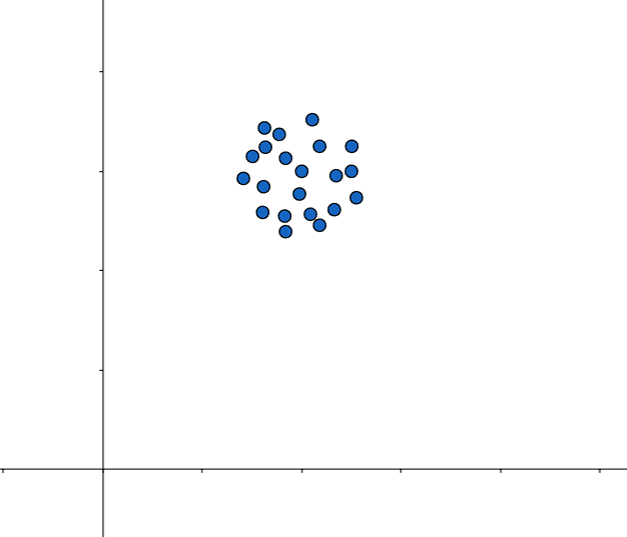
\includegraphics[height=5cm]{mathstat/images/mathstat_2025_04_01_1}

            Здесь, возможно, нет зависимости

            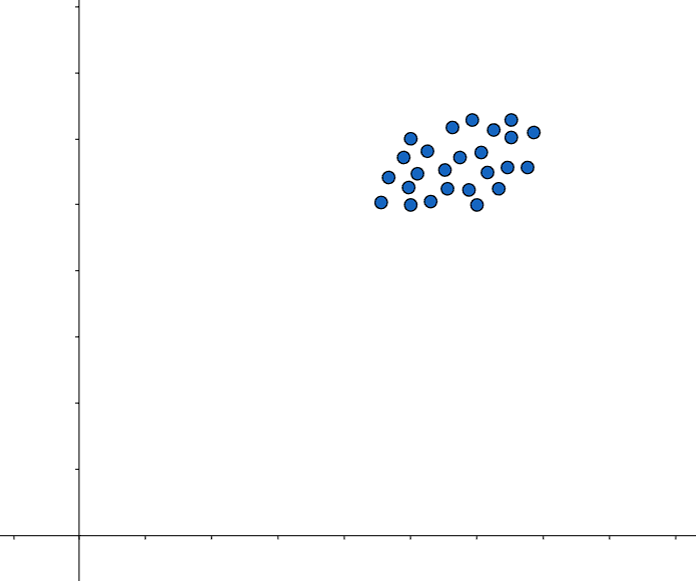
\includegraphics[height=5cm]{mathstat/images/mathstat_2025_04_01_2}

            Здесь можно предположить прямую корреляцию
        \end{center}
    \end{multicols}

    Пусть даны данные $X$ и $Y$ при $n$ экспериментов. Эти данные удобно представить в виде коррелеционной таблицы:
    по вертикали отмечают различные значения $x$, а по горизонтали - $y$, в клетках таблицы отмечаются частота появления $n_{xy}$

    \Ex $n = 50$

    \smallvspace

    \begin{tabular}{c|c|c|c|c|c|c}
        X\backslash Y & 10 & 20 & 30 & 40 & $n_x$ & $\overline y_x$ \\
        \hline
        2 & 7 & 3 & 0 & 0 & 10 & 13 \\
        \hline
        4 & 3 & 10 & 10 & 2 & 25 & 4.4 \\
        \hline
        6 & 0 & 2 & 10 & 3 & 15 & 30.67 \\
        \hline
        $n_y$ & 10 & 15 & 20 & 5 & $\Sigma$ 50 & \\
    \end{tabular}

    \smallvspace

    По диагонали таблицы можно предположить, что корреляция есть

    Имеет смысл вычислить условное среднее по формуле $\overline y (x) = \frac{1}{n_x} \sum n_{xy} y_i$. Так как в нашем примере
    условные средние растут с ростом $x$, то имеет место прямая корреляция

    \Notas Если данных много или $X$ и $Y$ -- непрерывные случайные величины, то лучше составить интервальную корреляционную таблицу:
    разбить случайные величины на интервалы, по вертикали отметить интервалы $[a_{i - 1}, a_i)$ случайной величины $X$, 
    по горизонтали -- $[b_{j - 1}, b_j)$ случайной величины $Y$, в клетках 
    отметить частоты $n_{ij} : [a_{i - 1}, a_i) \times [b_{j - 1}, b_j)$. В дальнейшем интервалы можно заменить их серединами

    \item Критерий хи-квадрат для проверки независимости.

    \hyperlink{chi_square_independence_criterion}{Критерий хи-квадрат для проверки независимости}
    
    Пусть выборка $(X_1, Y_1), (X_2, Y_2), \dots, (X_n, Y_n)$ представлена в виде интервальной корреляционной таблицы. Случайная величина $X$ 
    разбита на $k$ интервалов, а $Y$ -- на $m$ интервалов

    Обозначим $v_{i\cdot}$ -- частота $i$-ого интервала $[a_{i - 1}, a_i)$ случайной величины $X$, 
    $v_{\cdot j}$ -- частота $j$-ого интервала $[b_{j - 1}, b_j)$ случайной величины $Y$, $v_{ij}$ -- число точек в $[a_{i - 1}, a_i) \times [b_{j - 1}, b_j)$


    \begin{tabular}{c|c|c|c|c|c}
        X\backslash Y & $[b_0, b_1)$ & $[b_1, b_2)$ & \dots & $[b_{m - 1}, b_m)$ & $v_{i\cdot}$ \\
        \hline
        $[a_0, a_1)$ & $v_{11}$ & $v_{12}$ & \dots & $v_{1m}$ & $v_{1\cdot}$ \\
        \hline
        \multicolumn{6}{c}{\dots} \\
        \hline
        $[a_{k - 1}, a_k)$ & $v_{k1}$ & $v_{k2}$ & \dots & $v_{km}$ & $v_{k\cdot}$ \\
        \hline
        $v_{\cdot j}$ & 10 & 15 & 20 & 5 & $\Sigma n$ \\
    \end{tabular}

    Проверяется основная гипотеза $H_0 : X \text{ и } Y$ независимы против $H_1 = \overline{H_0} : X \text{ и } Y$ зависимы

    Если $H_0$ верна, то $p_{ij} = P(X \in [a_{i - 1}, a_i), Y \in [b_{j - 1}, b_j)) = P(X \in [a_{i - 1}, a_i)) \cdot P(Y \in [b_{j - 1}, b_j))$

    Тогда по закону больших чисел $\frac{v_{i\cdot}}{n} \ConvergesInProbability p_{i\cdot}, \frac{v_{\cdot j}}{n} \ConvergesInProbability p_{\cdot j}$

    Поэтому основанием для отклонения основной гипотезы будет заметная разница между величинами $\frac{v_{i\cdot}}{n}\frac{v_{\cdot j}}{n}$ и 
    $\frac{v_{ij}}{n}$ или $v_{ij}$ и $\frac{1}{n} v_{i\cdot} v_{\cdot j}$

    В качестве статистики берется $K = n \sum_{i, j} \frac{\left(v_{ij} - \frac{1}{n} v_{i\cdot} v_{\cdot j}\right)^2}{v_{i\cdot} v_{\cdot j}}$

    \begin{MyTheorem}
        \Ths Если $H_0$ верна, то $K \rightrightarrows H_{(k - 1)(m - 1)}$
    \end{MyTheorem}

    Пусть $t_\alpha$ -- квантиль $H_{(k - 1)(m - 1)}$ уровня $\alpha$, тогда 

    \begin{cases}
        H_0 : X \text{ и } Y \text{ независимы, если } K < t_\alpha \\
        H_0 : X \text{ и } Y \text{ зависимы, если } K \geq t_\alpha \\
    \end{cases}

    \Nota Для работы критерия необходимо, что бы частота в каждой клетке была больше 5, а объем выборки был достаточно большой

    \item Однофакторный дисперсионный анализ. Общая, межгрупповая и внутригрупповая дисперсии. Теорема о разложении дисперсии.

    Для каждой выборки вычислим выборочное среднее и дисперсию: $\overline{x}^{(j)} = \frac{1}{n_j} \sum_{i = 1}^{n_j} X_i^{(j)}$, 
    $D^{(j)} = \frac{1}{n_j} \sum_{i = 1}^{n_j} (X_i^{(j)} - \overline{x}^{(j)})^2$

    Объединим все выборки в общую и также вычислим выборочнее среднее и дисперсию: 

    $\overline{x} = \frac{1}{n} \sum_{i, j} x^{(j)}_i = \frac{1}{n} \sum_{j = 1}^k n_j \cdot \overline{x}^{(j)}$ - общее среднее

    $D_\text{О} = \frac{1}{n} \sum_{i, j} (X^{(j)}_i - \overline{x})^2$ - общая дисперсия

    \Def Внутригрупповой (или остаточной) дисперсией называется среднее групповых дисперсий: $D_{\text{В}} = \frac{1}{n} \sum_{j = 1}^k n_j D^{(j)}$

    \Def Межгрупповой (или факторной) дисперсией называется величина $D_{\text{М}} = \frac{1}{n} \sum_{j = 1}^k n_j (\overline{x} - \overline{x}^{(j)})^2$

    \begin{MyTheorem}
        \ThNs{О разложении дисперсии} Общая дисперсия равна сумме внутригрупповой и межгрупповой дисперсией: $D_\text{О} = D_\text{В} + D_\text{М}$
    \end{MyTheorem}

    Смысл: внутригрупповая дисперсия показывает средний (случайный) разброс внутри выборок, межгрупповая - насколько отличаются среднее при различных 
    уровнях фактора, то есть именно эта величина отражает влияния фактора

    Вывод по наличии корреляции можно сделать, если доля $D_\text{М}$ достаточно велика

    \item Однофакторный дисперсионный анализ. Проверка гипотезы о влиянии фактора.

    \hyperlink{factor_influence_hypothesis}{Проверка гипотезы о влиянии фактора}
    
    Предполагаем, что $X$ имеет нормальное распределение и фактор $Z$ может влиять только на ее математическое ожидание, 
    но не на дисперсию и тип распределения, поэтому можно считать, что данные независимых $k$ выборок при различных уровнях фактора $Z$
    также имеют нормальное распределение с одинаковой дисперсией: $X^{(j)} \in N(a_j, \sigma^2)$

    Проверяется основная гипотеза $H_0 : a_1 = a_2 = \dots = a_k$ (фактор не оказывает влияния) против $H_1 = \overline{H_0} : $ есть влияние

    По пункту 3 основной теоремы $\sum_{i = 1}^n \left(\frac{x_i - \overline{x}}{\sigma}\right)^2 = \frac{n D^*}{\sigma^2} \in H_{n - 1}$

    Из этого $\frac{n_j D^{(j)}}{\sigma^2} \in H_{n_j - 1} \quad \forall \ 1 \leq j \leq k$

    Так как распределение \enquote{хи-квадрат} устойчиво относительно суммирования, то $\sum_{j = 1}^k \frac{n_j D^{(j)}}{\sigma^2} \in H_{n - k}$, так как
    $(n_1 - 1) + \dots + (n_k - 1) = n - k$

    Пусть основная гипотеза верна, тогда все данные можно считать выборкой одной случайной величины и по пункту 3 $\frac{n D_{\text{О}}}{\sigma^2} \in H_{n - 1}$

    Согласно теореме о разложении дисперсии $D_\text{О} = D_\text{В} + D_\text{М}$, тогда $\frac{n D_{\text{О}}}{\sigma^2} = \frac{n D_{\text{В}}}{\sigma^2} + \frac{n D_{\text{М}}}{\sigma^2}$

    Так как $\frac{n D_{\text{О}}}{\sigma^2} \in H_{n - 1}, \frac{n D_{\text{В}}}{\sigma^2} \in H_{n - k}$, то $\frac{n D_{\text{М}}}{\sigma^2} \in H_{k - 1}$

    Тогда при верной основной гипотезе получим, что $\frac{n D_{\text{М}}}{\sigma^2} \frac{\sigma^2 (n - k)}{n D_\text{В}} = \frac{n - k}{k - 1} \frac{D_\text{М}}{D_\text{В}} \in F(k - 1, n - k)$ --
    распределение Фишера-Снедекера со степенями $k - 1$ и $n - k$

    В качестве статистики берется $K = \frac{n - k}{k - 1} \frac{D_\text{М}}{D_\text{В}}$, в качестве критической точки $t_\alpha$ -- квантиль $F(k - 1, n - k)$ уровня $\alpha$

    \begin{cases}
        H_0 : a_1 = a_2 = \dots = a_k \text{ (фактор не оказывает влияние), если } K < t_\alpha \\
        H_1 : \text{фактор влияние оказывает, если } K \geq t_\alpha \\
    \end{cases}

    \item Математическая модель регрессии. Основные понятия и определения. Метод наименьших квадратов.

    Пусть случайная величина $X$ зависит от случайной величины $Z$ (необязательно случайной)

    \Def \hyperlink{regression}{Регрессией} $X$ на $Z$ называется функция $f(z) = E(X|Z = z)$. 
    Она показывает зависимость среднего значения $X$ от значения $Z$

    Уравнение $x = f(z)$ называется уравнением регрессии, а график этой функции - линия регрессии

    Пусть при $n$ экспериментах при значениях $Z_1, Z_2, \dots, Z_n$ фактора $Z$ наблюдались значения
    $X_1, X_2, \dots, X_n$ случайной величины $X$

    Обозначим через $\varepsilon_i$ разницу между экспериментальным и теоретическими значениями случайной величины $X$,
    то есть $\varepsilon_i = X_i - f(z_i)$

    $\varepsilon$ - это случайный член модели или так называемая теоретическая ошибка

    \Nota Обычно можно считать, что $\varepsilon_i$ независимы друг от друга и имеет нормальное распределение с $a = 0$,
    так как $E\varepsilon_i = E(X_i - f(Z_i)) = E(X | Z = Z_i) - E(X | Z = Z_i) = 0$

    Цель: нам нужно по экспериментальным данным $(z_1, x_1), \dots, (z_n, x_n)$ как можно лучше оценить функцию $f(z)$

    \Notas При этом предполагая (часто из теории), что $f(z)$ - функция определенного вида, но параметры которой неизвестны.
    Если нет, то начинаем подбирать модели самого простого вида. В противном случае, наилучшим решением была бы кривая, 
    проходящая через все точки 

    \hyperlink{method_of_least_squares}{Метод наименьших квадратов}:

    Пусть известен из теории вид функции $f(z)$. Метод наименьших квадратов состоит в выборе параметров $f(z)$ таким образом,
    чтобы минимизировать сумму квадратов ошибок $\sum_{i = 1}^n \varepsilon_i^2 = \sum_{i = 1}^n (X_i - f(Z_i))^2 \rightarrow \min$

    \Def Пусть $\theta$ - набор неизвестных параметров функции $f(z)$. Оценка $\hat \theta$ параметра $\theta$, 
    при которой достигается минимум $\sum_{i = 1}^n \varepsilon_i^2$, называется оценкой метода наименьших квадратов (или ОМНК)

    \item Вывод уравнения линейной парной регрессии. Геометрический смысл прямой регрессии.

    
    Пусть имеется теоретическая модель линейной регрессии: $f(z) = \alpha + \beta z + \varepsilon$ - теоретическая модель, где $\varepsilon$ - теоретическая ошибка
    отражающая влияние невключенных в модель факторов, возможной нелинейности, ошибок измерения и просто случая

    Пусть $(z_1, x_1), \dots, (z_n, x_n)$ - экспериментальные данные. По ним методом наименьших квадратов строим
    экспериментальную модель линейной регрессии $f(z) = a + b z$, где $a$ и $b$ - ОМНК параметров $\alpha$ и $\beta$

    $\hat \varepsilon_i = X_i - f(Z_i) = X_i - (a + b Z_i)$ - экспериментальная ошибка

    Найдем ОМНК параметров $\alpha$ и $\beta$

    $\sum_{i = 1}^n \hat \varepsilon_i^2 = \sum_{i = 1}^n (X_i - (a + b Z_i))$

    $\frac{\partial}{\partial a} \sum_{i = 1}^n \hat \varepsilon_i^2 = \sum_{i = 1}^n -2 (X_i - a - b Z_i) = 
    -2 \sum_{i = 1}^n X_i + 2\sum_{i = 1}^n a + 2b \sum_{i = 1}^n Z_i = -2(n \overline{x} - na - bn \overline{z})$

    $\frac{\partial}{\partial b} \sum_{i = 1}^n \hat \varepsilon_i^2 = \sum_{i = 1}^n -2 Z_i (X_i - a - b Z_i) = 
    -2 \sum_{i = 1}^n X_i Z_i + 2\sum_{i = 1}^n a Z_i + 2b \sum_{i = 1}^n Z_i^2 = -2(n \overline{x z} - a n \overline{z} - bn \overline{z^2})$

    \begin{cases}
        -2 (n \overline{x} - na - nb \overline{z}) = 0 \\
        -2 (n \overline{zx} - na \overline{z} - nb \overline{z^2}) = 0 \\
    \end{cases} $\Longleftrightarrow$ \begin{cases}
        a + b\overline{z} = \overline{x} \\
        a\overline{z} + b \overline{z^2} = \overline{zx} \\
    \end{cases} 

    Получили систему линейных уравнений. Будем называть ее нормальной системой. При решении получаем:

    \begin{cases}
        a = \overline{x} - b \overline{z} \\
        (\overline{x} b \overline{z}) \overline{z} + b \overline{z^2} = \overline{zx} \\
    \end{cases} $\Longleftrightarrow$ \begin{cases}
        a = \overline{x} - b \overline{z} \\
        b = \frac{\overline{zx} - \overline{z} \, \overline{x}}{\hat \sigma^2_z}
    \end{cases} - ОМНК 

    Запишем уравнение линейной регрессии в удобном виде: $\overline{x}_z = f(z) = E(X | Z = z)$

    $\overline{x}_z = a + bz$

    $\overline{x}_z = \overline{x} - b \overline{z} + bz$

    $\overline{x}_z - \overline{x} = \frac{\overline{z x} - \overline{x} \, \overline{z}}{\hat \sigma^2_z} (z - \overline{z})$

    $\overline{x}_z - \overline{x} = \frac{\hat \sigma_x}{\hat \sigma_z} \frac{\overline{z x} - \overline{x} \, \overline{z}}{\hat \sigma_z \hat \sigma_x} (z - \overline{z}) = 
    \frac{\hat \sigma_x}{\hat \sigma_z} \hat r (z - \overline{z})$, где $\hat r$ - выборочный коэффициент линейной корреляции

    Или $\frac{\overline{x}_z - \overline{x}}{\hat \sigma_x} = \hat r \frac{z - \overline{z}}{\hat \sigma_z}$ - выборочное уравнение линейной регрессии

    \begin{center}
        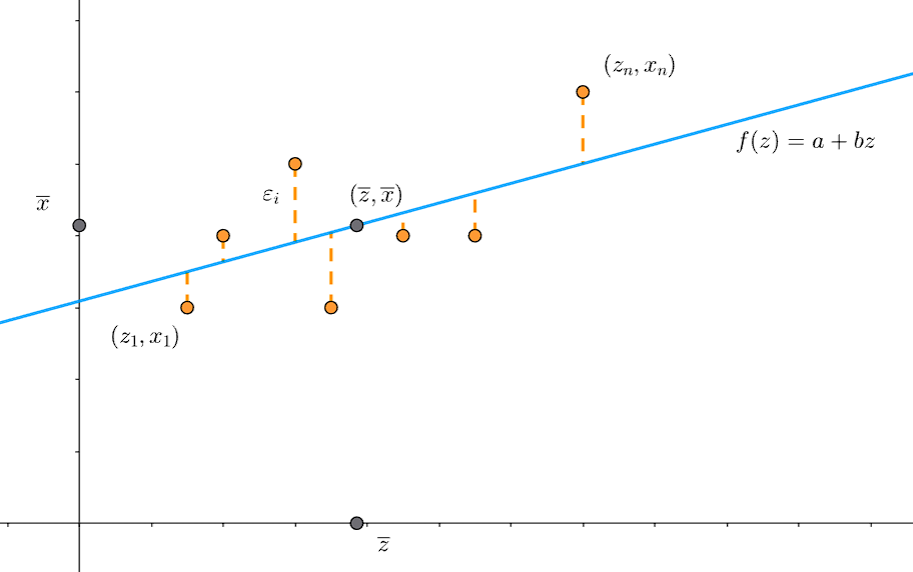
\includegraphics[height=7cm]{mathstat/images/mathstat_2025_04_08_1}
    \end{center}

    Суть МНК: находим такую прямую, чтобы сумма квадратов длин этих отрезков (по сути отклонений) была минимальна 
    (или дисперсия экспериментальных данных относительно прямой была минимальна)

    \item Выборочный коэффициент линейной корреляции. Проверка гипотезы о его значимости.

    \Def $\hat r = \frac{\overline{z x} - \overline{x} \, \overline{z}}{\hat \sigma_z \hat \sigma_x}$ называется \hyperlink{selective_coefficient_linear_correlation}{выборочным коэффициентов 
    линейной корреляции}. Ясно, что она будет точечной оценкой теоретического коэффициента линейной корреляции. 
    Также $\hat r$ является несмещенной оценкой

    Поэтому выборочный коэффициент корреляции характеризует силу линейной связи. Знак коэффициента показывает направления корреляции (прямая или обратная)

    Пусть $(Z, X)$ распределена нормально. По выборке объема $n$ вычислен выборочный коэффициент корреляции $\hat r$, а $r$ - теоретический коэффициент корреляции

    Проверяется $H_0 : r = 0$ (выборочный коэффициент корреляции статистически незначим) против $H_1 : r \neq 0$ (коэффициент статистически значим)

    \begin{MyTheorem}
        Если $H_0$ верна, то $K = \frac{\hat r \sqrt{n - 2}}{\sqrt{n - \hat r^2}} \in T_{n - 2}$ - распределение Стьюдента с степенью $n - 2$ 
    \end{MyTheorem}

    Получаем критерий. Пусть $t_\alpha$ - квантиль $|T_{n - 2}|$ (двухстороннее распределение Стьюдента) уровня $\alpha$

    \begin{cases}
        H_0 : r = 0, & \text{ если } |K| < t_\alpha \\
        H_1 : r \neq 0, & \text{ если } |K| \geq t_\alpha \\
    \end{cases}

    \item Выборочное корреляционное отношение, его свойства.

    Пусть есть $k$ выборок случайной величины $X$ при $k$ различных уровнях фактора $Z$. Вычислены общая, внутригрупповая и межгрупповая дисперсии. 
    По теореме $D_\text{О} = D_\text{М} + D_\text{В}$

    \Def \hyperlink{selective_correlational_relation}{Выборочным корреляционным отношением} $X$ на $Z$ называется величина $\eta_{X, Z} = \sqrt{\frac{D_\text{М}}{D_\text{О}}}$

    \underline{Свойства}:

    \begin{enumerate}
        \item $0 \leq \eta_{X, Z} \leq 1$ ($D_\text{М}, D_\text{О} \geq 0$)

        \item Если $\eta = 1$, то $D_\text{М} = D_\text{О} \Longrightarrow D_\text{В} = 0$, имеем функциональную зависимость $X$ от $Z$

        \item Если $\eta = 0$, то $D_\text{М} = 0 \Longrightarrow$ корреляция отсутствует

        \item $\eta \geq |\hat r|$

        \item Если $\eta = |\hat r|$, то все точки экспериментальных данных лежат на прямой линейной регрессии 
        (то есть данная линейная модель является идеальной)

    \end{enumerate}

    \item Свойства ошибок в модели линейной парной регрессии. Анализ дисперсии фактора-результата. Коэффициент детерминации, его свойства.

    Пусть при $n$ экспериментах получены значения случайных величин $X$ и $Z$: $(X_1, Z_1), \dots, (X_n, Z_n)$

    Пусть $X = \alpha + \beta Z + \varepsilon$ - теоретическая модель линейной регрессии, где $\varepsilon$ - случайная величина,
    отражающая влияние невключенных факторов, нелинейность модели, ошибок измерений и просто случая.

    Пусть построили с помощью метода наименьших квадратов выборочное уравнение линейной регрессии $\hat X = a + b Z$

    Обозначим $\hat \varepsilon_i = X_i - \hat X_i$ - экспериментальная ошибка, разница между наблюдаемыми значениями и 
    вычисляемыми по модели

    Тогда $X_i = \hat X_i + \hat \varepsilon_i$ или $X_i = a + b Z_i + \hat \varepsilon_i$, где $a$ и $b$ - точечные оценки параметров $\alpha$ и $\beta$

    Свойства $\hat \varepsilon_i$:

    \begin{enumerate}
        \item $\overline{\hat \varepsilon_i} = 0$

        \begin{MyProof}
            $a = \overline{X} - b \overline{Z} \Longrightarrow a + b \overline{Z} = \overline{X} \Longrightarrow \overline{\hat \varepsilon_i} = \overline{X_i - (a + b Z_i)} = \overline{X} - \overline{a + b Z_i} = \overline{X} - \overline{X} = 0$
        \end{MyProof}

        \item $\cov (\hat X, \hat \varepsilon) = 0$

        \begin{MyProof}
            $b = \overline{\overline{xz} - \overline{x} \cdot \overline{z}}{\hat \sigma^2_z} = \overline{\cov (X, Z)}{D(Z)} \Longrightarrow \cov (X, Z) - b D(Z) = 0$

            $\cov (\hat X, \hat \varepsilon) = \cov (a + b Z, X - a - bZ) = \cov (bZ, X - bZ) = \cov (bZ, x) - \cov (bZ, bZ) = b \cov (Z, X) - b^2 D(Z) = b (\cov (Z, X) - b D(Z)) = 0$
        \end{MyProof}
    \end{enumerate}

    \Def $D(X) = \frac{1}{n} \sum_{i = 1}^n (X_i - \overline{X})^2$ - дисперсия наблюдаемых значений

    \Defs $\hat D(X) = \frac{1}{n} \sum_{i = 1}^n (\hat X_i - \overline{X})^2$ - дисперсия расчетных значений

    \Defs $D(\hat \varepsilon) = \frac{1}{n} \sum_{i = 1}^n (\hat \varepsilon_i)^2$ - дисперсия остатков

    Так как $X = \hat X + \hat \varepsilon$, $\cov (\hat X, \hat \varepsilon) = 0$, то $D(X) = D(\hat X) + D(\hat \varepsilon) + 2\cov (\hat X, \hat \varepsilon) = D(\hat X) + D(\hat \varepsilon)$

    \begin{MyTheorem}
        \Ths $D(X) = D(\hat X) + D(\hat \varepsilon)$
    \end{MyTheorem}

    Очевидно, что качество модели будет тем лучше, чем меньше будет дисперсия остатков

    \Def Коэффициентом детерминации $R^2$ называется величина $R^2 = \frac{D(\hat X)}{D(X)}$ или $R^2 = 1 - \frac{D(\hat \varepsilon)}{D(X)}$

    \Notas Смысл $R^2$ - доля объясненной дисперсии, а $1 - R^2$ - доля необъясненной дисперсии

    Свойства: 

    \begin{enumerate}
        \item $0 \leq R^2 \leq 1$
        \item Если $R^2 = 1$, то $D(\hat \varepsilon) = 0 \Longrightarrow \hat \varepsilon_i = \overline{\hat \varepsilon_i} = 0$, то есть точки лежат строго на 
        линии регрессии, модель идеальна

        \item Если $R^2 = 0$, то $D(\hat X) = 0 \Longrightarrow \hat X = \overline{x}$, то есть получаем примитивную, ничего не объясняющую модель
    \end{enumerate}

    Чем больше $R^2$, тем лучше качество модели

    \item Проверка гипотезы о значимости уравнения линейной регрессии. Связь между коэффициентом детерминации и коэффициентом линейной корреляции.

    \hyperlink{linear_regression_hypothesis}{Проверка гипотезы о значимости уравнения линейной регрессии}: проверяется $H_0 : R^2_\text{теор} = 0$ (уравнение регрессии статистически не значимо) против $H_1 : R^2_\text{теор} \neq 0$

    \begin{MyTheorem}
        \Ths Если $H_0$ верна, то $F = \frac{R^2 (n - 2)}{1 - R^2} \in F(1, n - 2)$
    \end{MyTheorem}

    Пусть $t_\alpha$ - квантиль $F(1, n - 2)$ уровня $\alpha$, тогда:

    \begin{cases}
        H_0 : R^2_{\text{теор}} = 0 & \text{ если } F < t_\alpha \\
        H_0 : R^2_{\text{теор}} \neq 0 & \text{ если } F \geq t_\alpha \\
    \end{cases}

    \Nota Если $H_0 : R^2_{\text{теор}} = 0$, то $H_0 : \beta = 0$

    \hyperlink{correlation_coefficient_connection}{Связь между коэффициентом детерминации и коэффициентом линейной корреляции}{}

    \begin{enumerate}
        \item $\sqrt{R^2} = r_{\hat X, X}$ - коэффициент корреляции между $\hat X$ и $X$
        \begin{MyProof}
            $r_{\hat X, X} = \frac{\cov (\hat X, X)}{\sqrt{D(\hat X) D(X)}} = \frac{\cov (\hat X, \hat X + \hat \varepsilon)}{\sqrt{D(\hat X) D(X)}} = 
            \frac{D(\hat X) + \cancelto{0}{\cov (\hat X, \hat \varepsilon)}}{\sqrt{D(\hat X) D(X)}} = \sqrt{\frac{D(\hat X)}{D(X)}} = R$
        \end{MyProof}

        \item $r_{\hat X, X} = |r_{X, Z}|$

        \begin{MyProof}
            $\cov (\hat X, X) = \cov (a + bZ, X) = b \cov (Z, X)$

            $D(\hat X) = D(a + b Z) = b^2 D(Z)$

            $r_{\hat X, X} = \frac{\cov (\hat X, X)}{\sqrt{D(\hat X) D(X)}} = \frac{b \cov (Z, X)}{\sqrt{b^2 D(Z) D(X)}} = \left|\frac{\cov (X, Z)}{\sqrt{D(Z) D(X)}}\right| = |r_{X, Z}|$
        \end{MyProof}
    \end{enumerate}

    \item Теорема Гаусса-Маркова.

    \begin{MyTheorem}
        \ThNs{\hyperlink{gauss_markov_theorem}{Теорема Гаусса-Маркова}} Пусть $X_i = \alpha + \beta Z_i + \varepsilon_i$ - теоретическая модель регрессии

        $X = a + b Z$ - модель, полученная по методу наименьших квадратов

        Если выполнено условия:

        \begin{enumerate}[label=\asbuk*),ref=\asbuk*]
            \item Случайные члены $\varepsilon_i$ независимые случайные величины, имеющие одинаковое нормальное распределение $\varepsilon_i \in N(0, \sigma^2)$
            \item Случайные величины $\varepsilon_i$ и $Z_i$ - независимы
        \end{enumerate}

        Тогда $a$ и $b$ - состоятельные, несмещенные, эффективные оценки параметров $\alpha$ и $\beta$, то есть

        \begin{enumerate}
            \item Состоятельность: $a \underset{n \to \infty}{\ConvergesInProbability} \alpha, b \underset{n \to \infty}{\ConvergesInProbability} \beta$
            \item Несмещенность: $Ea = \alpha, Eb = \beta$
            \item Наименьшая дисперсия, равная:

            $D a = \frac{\overline{z^2} \sigma^2}{n D(Z)}, Db = \frac{\sigma^2}{n D(Z)}$
        \end{enumerate}
    \end{MyTheorem}


    \item Стандартные ошибки коэффициентов регрессии. Их доверительные интервалы.

    Из теоремы видим, что $Da$ и $Db$ зависят от дисперсии $\sigma^2$ случайного члена. 
    По экспериментальным ошибкам получаем оценку данной дисперсии:

    $D(\hat \varepsilon) = \frac{1}{n} \sum_{i = 1}^n {\hat \varepsilon_i}^2 \underset{n \to \infty}{\ConvergesInProbability} \sigma^2$

    Однако эта оценка является смещенной: $E(D(\hat \varepsilon)) = \frac{n - 2}{n} \sigma^2$

    Поэтому несмещенной оценкой дисперсии $\sigma^2$ является величина $S^2 = \frac{1}{n - 2} \sum_{i = 1}^n {\hat \varepsilon_i}^2$

    \Def Величина $S$ называется \hyperlink{regression_coefficient_error}{стандартной ошибкой регрессии}

    Смысл: характеризует разброс наблюдаемых значений вокруг линии регрессии

    \Notas Заменим в теореме Гаусса-Маркова $\sigma^2$ на $S^2$, получаем оценки дисперсий $Da$ и $Db$: $S_a^2 = \frac{\overline{z^2} S^2}{n D(z)}, S^2_b = \frac{S^2}{n D(Z)}$

    \Defs $S_a$ и $S_b$ называются стандартным ошибками коэффициентов регрессии

    Пусть $t_\gamma$ - квантиль $|T_{n - 2}|$ уровня $\gamma$

    Тогда доверительные интервалы надежности $\gamma$ для параметров $\alpha$ и $\beta$:

    $\qquad \alpha: (a - t_\gamma S_a; a + t_\gamma S_a)$

    $\qquad \beta: (b - t_\gamma S_b; b + t_\gamma S_b)$

    \item Прогнозирование в модели линейной парной регрессии. Стандартная ошибка прогноза, доверительный интервал прогноза.

    Пусть $X = \alpha + \beta Z + \varepsilon$ - теоретическая модель

    $\hat X = a + b Z$ - модель МНК, построенная по выборке объема $n$

    С помощью данной модели надо дать прогноз значения $X_p$ при заданном значении $Z_p$ и оценить качество прогноза 

    Теоретическое значение - $X_p = \alpha + \beta Z_p + \varepsilon$, а точечный прогноз $\hat X_p = a + b Z_p$

    Разность между ними $\Delta_p = \hat X_p - X_p$ называется ошибкой предсказания

    Свойства $\Delta_p$:

    \begin{enumerate}
        \item $E \Delta_p = 0$
        \item $D (\Delta_p) = \left(1 + \frac{1}{n} + \frac{(Z_p - \overline{z})^2}{n DZ}\right) \sigma^2$

        Заменив $\sigma^2$ на $S^2$, получим стандартную ошибку прогноза: $S_{\Delta_p} = S \sqrt{1 + \frac{1}{n} + \frac{(Z_p - \overline{z})^2}{n DZ}}$

        \item $D(\Delta_p) > \sigma^2$ - то есть точность прогноза ограничена случайным членом $\varepsilon$

        \item При $n \to \infty$ $D(\Delta_p) \ConvergesInProbability \sigma^2$ - качество модели тем лучше, чем больше объем выборки

        \item Чем больше $Z_p$ отклоняется от $\overline{z}$, тем хуже качество прогноза. Наилучшее качество в точке $Z_p = \overline{z}: \ D(\Delta_p) = \left(1 + \frac{1}{n}\right) \sigma^2$

        % https://www.geogebra.org/calculator/brxkjkqc

        \begin{center}
            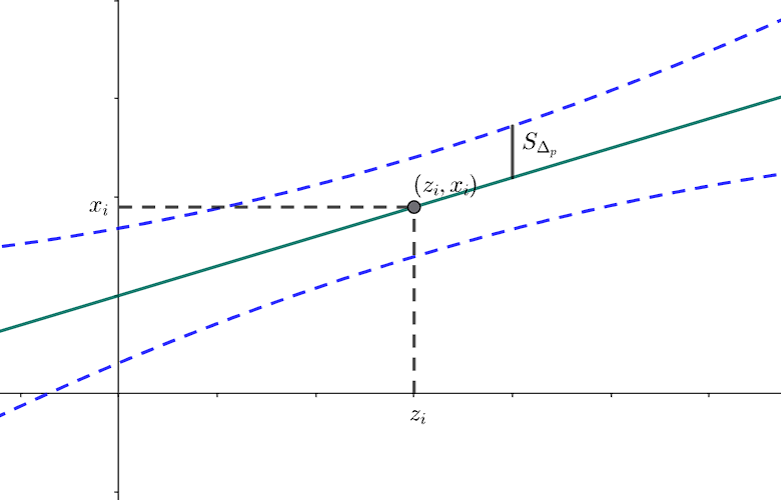
\includegraphics[width=7cm]{mathstat/images/mathstat_2025_04_15_1}
        \end{center}
    \end{enumerate}
    
    Доверительный интервал для прогноза $X_p: (\hat X_p - t_\gamma S_{\Delta_p}; \hat X_p + t_\gamma S_{\Delta_p})$

    \item Общая модель линейной регрессии. Вывод нормального уравнения.

    \hyperlink{general_regression}{Общая модель}: пусть результат $X$ зависит от $k$ факторов $Z_1, \dots, Z_k$. Рассматриваем теоретическую модель линейной регрессии:

    $X = \beta_1 Z_1 + \beta_2 Z_2 + \dots + \beta_k Z_k + \varepsilon$, где $\vec Z = \begin{pmatrix}Z_1 \\ \vdots \\ Z_k \end{pmatrix}$ - вектор факторов, $\vec \beta = \begin{pmatrix}\beta_1 \\ \vdots \\ \beta_k \end{pmatrix}$ - вектор коэффициентов регрессии

    Пусть проведено $n \geq k$ экспериментов, $\vec Z^{(i)} = \begin{pmatrix}Z_1^{(i)} \\ \vdots \\ Z_k^{(i)} \end{pmatrix}$ - значения факторов при $i$-ом эксперименте,
    $\vec X = \begin{pmatrix}X_1 \\ \vdots \\ X_n \end{pmatrix}$ - соответствующие значения результатов

    Согласно модели:

    \begin{cases}
        $X_1 = \beta_1 Z_1^{(1)} + \beta_2 Z_2^{(2)} + \dots + \beta_k Z_k^{(1)} + \varepsilon_1$ \\
        $X_1 = \beta_1 Z_1^{(1)} + \beta_2 Z_2^{(2)} + \dots + \beta_k Z_k^{(1)} + \varepsilon_1$ \\
        \dots \\
        $X_n = \beta_1 Z_1^{(n)} + \beta_2 Z_2^{(n)} + \dots + \beta_k Z_k^{(n)} + \varepsilon_n$
    \end{cases}

    Или в матричной форме: $\vec X = Z^T \vec \beta + \vec \varepsilon$, 
    где $Z = \begin{pmatrix}
        Z_1^{(1)} & Z_1^{(2)} & \dots & Z_1^{(n)} \\ 
        Z_2^{(1)} & Z_2^{(2)} & \dots & Z_2^{(n)} \\ 
        \vdots & \vdots & \ddots & \vdots \\
        Z_k^{(1)} & Z_k^{(2)} & \dots & Z_k^{(n)} \\ 
    \end{pmatrix}$ - матрица плана, $\vec \varepsilon$ - вектор теоретических ошибок

    Наша цель такова: по данной матрице плана $Z$ и вектора результатов $\vec X$ дать оценки неизвестных параметров регрессии $\beta_i$ 
    и параметров распределения ошибки $\varepsilon$

    Будем считать, что выполнено условие $\mathrm{Cond. 1}$, что ранг матрицы $\operatorname{rang} Z = k$, то есть все строки матрицы плана независимы

    Введем матрицу $A = Z Z^T$. Ее свойства:

    \begin{enumerate}
        \item $A$ - квадратная и симметричная
        \item $A$ - положительно определенная
        \item $\exists B = \sqrt{A}$, то есть $B^2 = A$
    \end{enumerate}

    Пусть $\vec B = \begin{pmatrix}b_1 \\ \vdots \\ b_k\end{pmatrix}$ - вектор оценок $\vec \beta = \begin{pmatrix}\beta_1 \\ \vdots \\ \beta_k\end{pmatrix}$

    Тогда эмпирическая модель регрессии $\vec{\hat X} = Z^T \vec B$, 
    $\vec \varepsilon_i = X_i - \hat X_i$ - экспериментальная ошибка, или $\vec {\hat \varepsilon} = \begin{pmatrix}\hat \varepsilon_1 \\ \vdots \\ \hat \varepsilon_n\end{pmatrix} = \vec X - Z^T \vec B$ - вектор экспериментальных ошибок

    По методу наименьших квадратов подбираем $\vec B$ таким образом, чтобы $L(\vec B) = \sum_{i = 1}^n \hat \varepsilon_i^2 \longrightarrow \min$

    $\sum_{i = 1}^n \hat \varepsilon_i^2 = \|\vec{\hat \varepsilon}\|^2 = \| \vec X - Z^T \vec B\|^2$ - квадрат расстояния от точки $\vec X$ до $Z^T \vec B$ в $\Real^n$

    $Z^T \vec B$ - точка линейного подпространства, порожденного векторами $Z^T \vec t$, где $\vec t \in \Real^k$

    \Nota Согласно $\mathrm{Cond. 1}$ размерность линейной оболочки, порожденной вектором $Z^T \vec t$,  $\dim \langle Z^T \vec t \rangle = k$

    Наименьшее расстояние получаем, когда квадрат расстояния от точки $\vec X$ до данного подпространства, а вектор $\vec B$ - проекция вектора $\vec X$ на него

    Таким образом, вектор $\vec X - Z^T \vec B$ должен быть ортогонален данному подпространству, то есть скалярное произведение вектора $\vec X$ и всех векторов подпространства равно 0

    $(Z^T \vec t, \vec X - Z^T \vec B) = (Z^T \vec t)^T (\vec X - Z^T \vec B) = {\vec t}^T (Z^T)^T (\vec X - Z^T \vec B) = {\vec t}^T Z (\vec X - Z^T \vec B) = 
    {\vec t}^T (Z \vec X - Z Z ^T \vec B) = 0 \ \forall \vec t \in \Real^k$

    Так как всем векторами подпространства ортогонален только нулевой вектор, то получаем, что $Z \vec X - Z Z^T \vec B = 0$ или $A \vec B = Z \vec X$ - нормальное уравнение (или система нормальных уравнений)

    Так как по свойству 2 матрица $A$ невырожденная, то существует обратная, получаем решение системы: $\vec B = A^{-1} Z \vec X$

    \item Свойства ОМНК в уравнении общей линейной регрессии.

    Добавим еще одно важное условие $\mathrm{Cond. 2}$: теоретические ошибки $\varepsilon_i$ - независимы и имеют одинаковое нормальное распределение $N(0, \sigma^2)$.
    То есть $E \vec \varepsilon = \vec 0$, $D \vec \varepsilon = \sigma^2 E_n$ (ковариации равны нулю в силу независимости)

    \underline{\hyperlink{mls_evaluation_properties}{Свойства}}:

    \begin{enumerate}
        \item $\vec B - \vec \beta = A^{-1} Z \vec \varepsilon$

        \begin{MyProof}
            $\vec B - \vec \beta = A^{-1} Z \vec X - \vec \beta = A^{-1} Z (Z^T \vec \beta + \vec \varepsilon) - \vec \beta = A^{-1} Z \vec \varepsilon$
        \end{MyProof}

        \item $\vec B$ - несмещенная оценка для вектора $\vec \beta$

        \begin{MyProof}
            $E(\vec B - \vec \beta) = E(A^{-1} Z \vec \varepsilon) = A^{-1} Z E \vec \varepsilon = 0 \Longrightarrow E \vec B = \vec \beta$
        \end{MyProof}

        \item Матрица ковариаций $D \vec B = \sigma^2 A^{-1}$

        \begin{MyProof}
            $D \vec B = D (\vec B - \vec \beta) = D (A^{-1} Z \vec \varepsilon) = A^{-1} Z D \vec \varepsilon A^{-1}^T Z^T = A^{-1} Z \sigma^2 E_n A^{-1}^T Z^T = \sigma^2 A^{-1} (Z Z^T) A^{-1} = \sigma^2 A^{-1}$
        \end{MyProof}

        Следствие: дисперсии оценок $b_i$ можно выразить через $\sigma^2$ и коэффициенты матрицы $A^{-1}$: $D b_i = \sigma^2 (A^{-1})_{ii}$

    \end{enumerate}

    \item Основная теорема об ОМНК (п.2 без доказательства).

    \begin{MyTheorem}
        Пусть выполнены $\mathrm{Cond. 1}$ и $\mathrm{Cond. 2}$, тогда $\frac{n \hat \sigma^2}{\sigma^2} \in H_{n - k}$ и не зависит от $\vec B$
    \end{MyTheorem}
    
    Так как $\frac{n \hat \sigma^2}{\sigma^2} \in H_{n - k}$, то $E \hat \sigma^2 = \frac{\sigma^2}{n} E \frac{n \hat \sigma^2}{\sigma^2} = \frac{\sigma^2}{n} (n - k) = \frac{n - k}{n} \sigma^2 < \sigma^2$ - смещенная вниз оценка
    
    Тогда несмещенной оценкой будет $S^2 = \frac{n}{n - k} \hat \sigma^2 = \frac{1}{n - k} \sum_{i = 1}^n \hat \varepsilon_i^2$

    \item Мультиколлинеарность, ее неприятные последствия. Основные принципы отбора факторов в модель общей линейной регрессии.
    \item Стандартная ошибка общей линейной регрессии и стандартные ошибки коэффициентов регрессии. Проверка гипотезы о значимости отдельного коэффициента регрессии.
    \item Уравнение регрессии в стандартных масштабах. Смысл стандартизованных коэффициентов. Разложение влияния фактора на прямое и косвенное.
    \item Коэффициенты детерминации и множественной корреляции, их свойства. Проверка гипотезы о значимости уравнения регрессии в целом.
    \item Взвешенный МНК.
    \item Приемы сведения нелинейных регрессий к линейным.
    \item Математические датчики случайных чисел.
    \item Моделирование случайных величин методом обратной функции (включая дискретный случай).
    \item Моделирование нормальной случайной величины.
    \item Быстрый показательный датчик.
    \item Моделирование дискретных случайных величин.
    \item Метод Монте-Карло. Общая постановка, оценка погрешности.
    \item Вычисление определенного и кратного интегралов методом Монте-Карло. Метод расслоенной выборки.
\end{enumerate}
